%% ============================================================
%% SELENE: Supportive Evidence-Based Oracles for Distributed Ledger Networks
%% Target: IEEE Journal of Biomedical and Health Informatics
%% ============================================================
%% COMPILE: pdflatex -> bibtex -> pdflatex -> pdflatex
%% ============================================================

\documentclass[journal]{IEEEtran}

%% --- Packages ---
\usepackage[T1]{fontenc}
\usepackage[utf8]{inputenc}
\usepackage{amsmath,amssymb,amsthm}
\usepackage{booktabs}
\usepackage{graphicx}
\usepackage{xcolor}
\usepackage{hyperref}
\usepackage{url}
\usepackage{cite}
\usepackage{multirow}
\usepackage{array}
\usepackage{tabularx}
\usepackage{balance}

%% --- Theorem environments ---
\newtheorem{theorem}{Theorem}
\newtheorem{lemma}{Lemma}
\newtheorem{proposition}{Proposition}
\newtheorem{corollary}{Corollary}
\theoremstyle{definition}
\newtheorem{definition}{Definition}
\theoremstyle{remark}
\newtheorem{remark}{Remark}

%% ============================================================
\begin{document}

\title{SELENE: Supportive Evidence-Based Oracles for\\
       Distributed Ledger Networks in Healthcare\\
       Claim Verification}

\author{First~Author,~\IEEEmembership{Member,~IEEE,}
        Second~Author,~\IEEEmembership{Senior Member,~IEEE,}
        and~Third~Author%
\thanks{Manuscript received \today.}%
\thanks{F. Author is with the Department of ...,
        University of ..., City, Country
        (e-mail: author@university.edu).}%
\thanks{S. Author and T. Author are with ...}}

\maketitle

%% ============================================================
%% ABSTRACT
%% Target: ~220 words. Five required elements:
%%   (1) Health informatics problem
%%   (2) Gap in existing work
%%   (3) Method and architecture
%%   (4) Concrete numerical results  <- fill \placeholder blocks
%%   (5) Clinical and domain significance
%% ============================================================
\begin{abstract}
Blockchain-based smart contracts are increasingly proposed
for healthcare claim verification, yet existing oracle designs
reduce heterogeneous clinical evidence to opaque scalar values,
obscuring how individual evidence sources contribute to
decisions and preventing meaningful audit.
Bayesian network~(BN)-based oracles address this by making
probabilistic reasoning explicit, but on-chain BN inference
incurs gas costs that grow with model size, limiting practical
deployability.
We present SELENE (Supportive Evidence-based oracles for distributed
LEdger NEtworks), a BN-based oracle architecture that resolves
this tension by anchoring BN parameters and evidence
assignments on-chain while executing inference off-chain,
preserving full post-hoc auditability without on-chain
computational overhead.
SELENE encodes posteriors in fixed-point form under a global
scale factor, manages claims through an explicit on-chain
state machine supporting incremental out-of-order evidence
arrival, and provides a complete reconstructible inference
transcript from ledger state alone.
We implement SELENE on Ethereum-compatible infrastructure
and evaluate a definitive four-contract deployment on the
Sepolia public testnet, with a separate parameterized
experiment measuring initialization scaling from 4 to
32 evidence nodes. On the production deployment,
\texttt{submitInference} consumed exactly
242{,}387~gas across 20 repetitions; its fixed-width
contract path is $O(1)$ with respect to BN inference
complexity. One-time CPT initialization scales linearly
at 53{,}492~gas per stored entry
($R^2{=}1.0000$). Fixed-point encoding under
$\texttt{SCALE}=10^6$ introduces a maximum absolute
error of $4.9688{\times}10^{-7}$ across 32 posterior
marginals, below the theoretical
$5{\times}10^{-7}$ bound, with no decision
inconsistencies.
We further establish, using information-measure bounds on
Bayesian risk, implementation-independent limits on how
reliable \emph{any} evidence-based oracle can be on a given
evidence channel, and derive a closed-form
privacy--reliability frontier under locally differentially
private evidence perturbation: for the studied
configuration, an $\varepsilon{\approx}1.10$ privacy budget
raises the attainable risk floor from $0.055$ to $0.232$.
These limits motivate a proposed risk-gating rule under
which a future contract could finalize a claim only once
the certified risk bound falls below an
application-defined tolerance.
Applied to physician-visit verification with four binary
evidence sources, SELENE demonstrates that interpretable,
auditable BN-based oracle decisions are practically
deployable in healthcare settings without prohibitive
on-chain costs, while identifying oracle centralization
and clinical CPT validation as the primary directions for
future work.
\end{abstract}

\begin{IEEEkeywords}
Bayesian inference, blockchain oracle, smart contracts,
healthcare informatics, gas optimization, evidence-based
reasoning, fixed-point arithmetic, claim verification
\end{IEEEkeywords}

%% ============================================================
\section{Introduction}
\label{sec:introduction}
%% ============================================================

\subsection{Motivation}

Smart contracts execute deterministically, yet their
correctness often depends on external data that contracts
cannot access directly.
As blockchain-based smart contracts increasingly mediate
high-stakes decisions in finance, supply chains, and
healthcare~\cite{hameed2024digital}, they rely on
\emph{oracles} to supply off-chain
information~\cite{sheldon2021auditing}.
This creates the \emph{oracle problem}: even with secure
on-chain consensus, contract correctness ultimately depends
on the trustworthiness and interpretability of off-chain
data feeds~\cite{pasdar2023connect,caldarelli2021blockchain},
a challenge examined across successive oracle surveys and
systematic
reviews~\cite{albreiki2020trustworthy,mammadzada2019review,gutierrez2024oracles,beniiche2020study}.

Most existing oracle designs address this by reducing
heterogeneous evidence to a scalar value: a price
feed~\cite{zhang2024blockchain,ahmadjee2025decision}, a
reputation
score~\cite{chen2022decentralized,nelaturu2020public,arshad2022reputable,
wang2025efficient}, or a majority
vote~\cite{adler2018astraea,sober2021voting}.
While sufficient for simple aggregation, scalar abstractions
obscure how individual evidence sources contribute to a
decision, making outcomes difficult to audit, contest, or
formally analyse~\cite{pasdar2023connect,ezzat2022blockchain}.
This limitation is especially consequential in healthcare,
where clinical and administrative decisions must
demonstrably follow from identifiable evidence, and where
regulatory frameworks increasingly require explainable,
auditable reasoning~\cite{eu_mdr_2017,goodman2017right}.

Bayesian Networks~(BNs) offer a principled alternative.
By representing claims and evidence as nodes and encoding
probabilistic dependencies via Conditional Probability
Tables~(CPTs), BNs enable structured, interpretable
inference in which each evidence source has an explicit
and locally verifiable effect on the posterior.
Prior work has demonstrated that BN-based reasoning can be
embedded directly in smart contracts, allowing on-chain
posterior computation from evidence~\cite{naeem2025evidence}.
This approach has two concrete advantages over scalar
oracles: decisions are derived from an explicit
probabilistic model whose parameters are visible on-chain,
and the contribution of each individual evidence source is
traceable through its CPT entries.

However, on-chain BN inference faces a fundamental
scalability barrier.
CPT evaluation and posterior normalization require
on-chain operations whose gas cost grows with the number
of evidence nodes, making full on-chain BN inference
impractical for models with more than a small number of
sources~\cite{naeem2025evidence}.
The obvious alternative---moving inference entirely
off-chain---reduces gas consumption but severs the
verifiability link: without a principled interface, smart
contracts cannot determine whether a reported posterior is
consistent with the BN parameters anchored to the ledger.
This creates a trust gap that existing designs do not
close.

The core tension is therefore this: on-chain BN inference
preserves verifiability but does not scale; off-chain
inference scales but abandons verifiability.
Neither extreme is acceptable for healthcare settings,
where both computational feasibility and decision
auditability are non-negotiable requirements.
A further complication is oracle centralization: if a
single operator controls inference submission, correctness
is assumed rather than enforced at execution time.
SELENE addresses this partially through on-chain parameter
anchoring and post-hoc auditability, but full
decentralization of the inference layer remains an open
problem scoped as future work.

These considerations motivate the following research
questions:

\begin{itemize}
  \item \textbf{RQ1:} Can a BN-based oracle be designed
  such that per-query on-chain gas cost is independent of
  BN size, while BN parameters, evidence assignments, and
  posterior outputs remain anchored and auditable on-chain?

  \item \textbf{RQ2:} Can a realistic claim--evidence
  lifecycle---in which claims are opened once and updated
  incrementally as evidence arrives out of order---be
  supported without contract redeployment or modification
  of the BN structure?

  \item \textbf{RQ3:} Does off-chain inference with
  on-chain parameter anchoring preserve sufficient
  numerical fidelity under fixed-point encoding that
  posteriors remain decision-consistent with their
  floating-point counterparts, and what are the conditions
  under which this guarantee holds?

  \item \textbf{RQ4:} Independently of any particular
  inference implementation, what is the \emph{fundamental}
  limit on the reliability of an evidence-based oracle
  given the statistical quality of its evidence channel,
  and how does that limit degrade when evidence must be
  privatised before being committed to a public ledger?
\end{itemize}

\subsection{Contributions}

This paper introduces \emph{SELENE} (Supportive Evidence-based oracles
for distributed LEdger NEtworks), a BN-based
oracle architecture that resolves the
scalability--verifiability tension by treating the
blockchain as an authenticated parameter and audit plane
rather than an inference engine.
Inference executes off-chain against a BN whose structure
and CPTs are anchored on-chain; only compact evidence
assignments and scaled posteriors are committed per query.
This keeps the on-chain interface fixed-width and
gas-predictable regardless of BN size, while preserving
the ability to reconstruct and independently verify every
inference decision from on-chain state.

The paper makes the following concrete contributions:

\begin{itemize}

  \item \textbf{Gas-predictable BN oracle architecture.}
  We design an oracle in which BN priors, CPTs, evidence
  states, and posterior outputs are anchored on-chain while
  inference executes off-chain. The production
  \texttt{submitInference} path is fixed-width and performs
  no BN inference or CPT traversal, giving $O(1)$ on-chain
  execution under the fixed query interface. On the
  definitive Sepolia deployment it consumes exactly
  242{,}387~gas across 20 repetitions, while a separate
  parameterized experiment shows that initialization scales
  linearly with CPT entries at 53{,}492~gas/entry
  ($R^2=1.0000$), in contrast with the size-dependent
  per-query cost inherent to full on-chain BN
  inference~\cite{naeem2025evidence}.

  \item \textbf{Formal evidence-based oracle model.}
  We define a restricted discrete BN with binary claim
  and evidence variables, derive a closed-form inference
  procedure, and specify a fixed-point encoding scheme.
  We characterise the rounding error introduced by
  fixed-point representation as a function of the scale
  factor and establish the conditions under which encoded
  posteriors remain decision-consistent with their
  floating-point counterparts.

  \item \textbf{Claim lifecycle and interaction protocol.}
  We specify and empirically evaluate an on-chain state
  machine supporting incremental, out-of-order evidence.
  Three claims are held concurrently in the
  \texttt{Open} state and updated under different evidence
  orderings. All 12 on-chain evidence records are
  independently reconstructed without error, all three
  orderings converge to the same complete-evidence
  posterior, and post-finalization updates revert in all
  three cases. Gas is stage-dependent but effectively
  invariant to evidence ordering at comparable stages.

  \item \textbf{Fundamental limits and a privacy
  frontier.}
  Casting oracle operation as Bayesian estimation, we
  derive implementation-independent lower bounds on the
  achievable risk of any evidence-based oracle in terms of
  maximal leakage and $\chi^2$-mutual information of its
  evidence channel, building on the information-measure
  framework of~\cite{esposito2024lower}. We show the
  bounds are monotone in the evidence set, derive from them
  a proposed \emph{risk-gating} predicate that certifies
  evidence sufficiency and could be enforced with
  constant-size contract logic, and use
  Strong Data-Processing Inequalities to obtain a
  closed-form trade-off between a local
  differential-privacy budget and attainable oracle
  reliability.

  \item \textbf{Implementation and empirical evaluation.}
  We deploy SELENE on Sepolia and evaluate gas,
  fixed-point fidelity, partial-evidence lifecycle
  behaviour, contract boundary conditions, and
  initialization scaling. \texttt{submitInference}
  consumes exactly 242{,}387~gas across 20 repeated
  production submissions; initialization scales at
  53{,}492~gas per CPT entry ($R^2=1.0000$); and the
  maximum fixed-point error is
  $4.9688\times10^{-7}$ with no decision
  inconsistencies across 32 marginals. CPT parameters are
  synthetic; clinical parameter validation remains future
  work.

\end{itemize}

Taken together, these contributions demonstrate that
interpretable, auditable BN-based oracle decisions are
practically deployable without gas costs that scale with
model complexity---a combination not achieved by prior
designs.
The architecture is explicit about its current
limitation: auditability is post-hoc, and the inference
layer remains centralized pending future work on
decentralized oracle committees.

The remainder of the paper is organized as follows.
Section~\ref{sec:relatedwork} reviews related work.
Section~\ref{sec:proposed-methodology} presents the SELENE
system model and BN formulation.
Section~\ref{sec:implementation} describes the
implementation.
Section~\ref{sec:experimental-analysis} reports
experimental results.
Section~\ref{sec:results-discussion} discusses trade-offs
and limitations.
Section~\ref{sec:conclusion} concludes.


%% ============================================================
\section{Related Work}
\label{sec:relatedwork}
%% ============================================================

Blockchain oracles provide external data to smart
contracts but differ significantly in how they aggregate
evidence, represent uncertainty, and ensure trust.
We survey four categories relevant to SELENE and summarize
key distinctions in Table~\ref{tab:oracle-comparison}.

\subsection{Data-Feed and Oracle Networks}

Widely deployed oracle systems such as
Chainlink~\cite{breidenbach2021chainlink} and
Witnet~\cite{de2017witnet} provide smart contracts
with scalar values---asset prices or event
outcomes---sourced from multiple off-chain providers.
These systems rely on aggregation mechanisms,
cryptographic signatures, and decentralized committees
to improve robustness against faulty or malicious data
providers~\cite{pasdar2023connect,ezzat2022blockchain,mammadzada2020blockchain}.
Foundational work has characterised how off-chain data is
brought on-chain in a trustworthy manner, formalising
inbound oracle patterns and data-on-chaining
systems~\cite{heiss2019oracles,muhlberger2020foundational}.
While effective for numerical feeds, such designs treat
inputs as atomic values and do not explicitly model how
different evidence sources contribute to a decision.
The reasoning process behind a reported value remains
implicit, limiting interpretability and making it
difficult to audit how individual signals affect
outcomes.

\subsection{Reputation, Voting, and Prediction-Market
Oracles}

Alternative oracle designs use economic incentives and
collective decision-making.
Reputation-based systems assign trust scores to data
providers~\cite{chen2022decentralized,nelaturu2020public,
arshad2022reputable}, while voting-based and
prediction-market oracles such as
Augur~\cite{peterson2015augur} aggregate reports through
token-weighted voting and reward mechanisms.
Kleros~\cite{lesaege2019kleros} extends this with
cryptoeconomic dispute resolution, and prediction markets
have themselves been studied as mechanisms for
probabilistic forecasting~\cite{shamsi2021prediction}.
These approaches provide economic security and
decentralization, but compress heterogeneous evidence
into scalar scores or discrete outcomes.
The relationship between individual evidence sources and
final decisions is not explicitly represented, limiting
transparency and making post-hoc analysis of decisions
difficult~\cite{pasdar2021blockchain}.

\subsection{Verifiable Computation and zk-Oracles}

A separate line of work focuses on verifiable
computation, in which off-chain results are accompanied
by cryptographic proofs verified on-chain.
Systems based on trusted execution environments such as
Town~Crier~\cite{zhang2016town} or zero-knowledge
proofs such as DECO~\cite{zhang2020deco} and
zk-SNARK-based oracles~\cite{garg2022succinct} ensure
that a reported output is consistent with a specified
computation.
These approaches provide strong correctness guarantees
but typically treat the underlying computation as a
black box.
While they can attest that a result was computed
correctly, they do not prescribe how to structure the
model itself or how to expose intermediate evidence and
parameters for interpretability.
Proof generation and verification also introduce
non-trivial overhead that scales with circuit complexity.
Related cryptographic machinery---succinct commitments with
fine-grained openings~\cite{kolonelos2023succinct},
incrementally verifiable
computation~\cite{datta2025incrementally}, and
oracle-based conditional
payments~\cite{madathil2022cryptographic}---further
illustrates the overhead and design complexity of
proof-carrying approaches relative to SELENE's
parameter-transparency model.

\subsection{Bayesian Network--Based Oracles}

Recent work explores the use of BNs to represent
structured evidence in oracle systems~\cite{naeem2025evidence}.
In these designs, claims and evidence are modeled
explicitly, and smart contracts compute posterior
probabilities directly from on-chain CPTs.
This enables interpretable, evidence-based decisions
with fully transparent parameters, consistent with the
broader use of Bayesian networks for structured reliability
and risk reasoning~\cite{wang2025application}.
However, executing BN inference on-chain incurs gas
costs that grow with the size of the network and the
number of evidence nodes, making such approaches
difficult to scale beyond small models.
Prior BN-based systems also remain largely
domain-agnostic decision aids; they do not address how
to commit BN parameters, evidence configurations, and
resulting decisions to a permissionless ledger in a
gas-efficient yet auditable manner.

\subsection{Information-Theoretic Limits of Estimation}

A separate literature establishes what \emph{cannot} be
achieved by any estimator, rather than proposing a
particular one. Classical treatments bound the Bayesian
risk through the Van Trees inequality and its
descendants, while information-theoretic approaches relate
achievable risk to the mutual information between the
parameter and the observations. Esposito \emph{et
al.}~\cite{esposito2024lower} generalise this programme to
essentially any information measure---R\'enyi's $\alpha$,
$\phi$-divergences, Sibson's $\alpha$-mutual information
and maximal leakage---by exploiting the duality between
spaces of measures and spaces of functions, and further
show how Strong Data-Processing Inequalities sharpen these
impossibility results when observations are privatised.

This literature has not previously been connected to
blockchain oracles, yet the fit is close. An oracle
consumes noisy, sparse or delayed observations of a latent
real-world state and must commit a decision; its evidence
sources form precisely an estimation channel. SELENE makes
that channel explicit and publicly auditable by anchoring
the CPTs on-chain, which is what allows the bounds
of~\cite{esposito2024lower} to be evaluated by any party
from ledger state alone
(Section~\ref{sec:theory-limits}). The same machinery
supplies the privacy--accuracy frontier that a public-ledger
deployment of a clinical oracle necessarily faces.

\subsection{Positioning SELENE}

SELENE occupies a distinct position in this landscape.
Unlike data-feed oracles, SELENE makes the probabilistic
model explicit: each evidence source is a node in a BN
whose CPTs are publicly anchored on-chain.
Unlike reputation and voting systems, SELENE produces
interpretable posteriors with a clear semantic link to
individual evidence sources.
Unlike verifiable computation approaches, SELENE does not
require proof generation; instead, it achieves
auditability through parameter transparency and
transcript completeness, trading runtime correctness
enforcement for architectural simplicity.
Unlike prior BN-on-chain designs, SELENE decouples
inference from the on-chain interface, achieving
gas-predictable operation regardless of BN size.
Table~\ref{tab:oracle-comparison} summarizes these
distinctions.

\begin{table}[t]
\centering
\caption{Comparison of oracle designs along inference,
accountability, and gas cost dimensions.}
\label{tab:oracle-comparison}
\resizebox{\columnwidth}{!}{%
\begin{tabular}{p{2.0cm}p{1.3cm}p{2.9cm}p{2.0cm}}
\toprule
\textbf{Category} &
\textbf{Inference} &
\textbf{Accountability} &
\textbf{Gas cost} \\
\midrule
Price / data-feed
oracles~\cite{breidenbach2021chainlink,
de2017witnet}
& Hybrid
& Values, signatures, committee votes
& Tied to feed size; model implicit \\
\addlinespace
Reputation / prediction-market
oracles~\cite{peterson2015augur,lesaege2019kleros}
& Off-chain / hybrid
& Reputation scores, staking, slashing, juror voting
& Depends on number of reporters \\
\addlinespace
Verifiable-computation
oracles~\cite{zhang2016town,zhang2020deco,
garg2022succinct}
& Off-chain
& Proofs on-chain; computation verifiable
& Proof generation cost \\
\addlinespace
BN-on-chain
oracles~\cite{naeem2025evidence}
& On-chain
& Parameters and posteriors fully on-chain
& Grows with BN size \\
\addlinespace
\textbf{SELENE (this work)}
& Off-chain
& Priors, CPTs, claim states, and per-claim
  posteriors recorded on-chain
& Per-query gas $\approx$ constant \\
\bottomrule
\end{tabular}}
\end{table}


%% ============================================================
\section{System Model and Architecture}
\label{sec:proposed-methodology}
%% ============================================================

SELENE treats the blockchain as an authenticated parameter
and audit plane rather than an inference engine.
A discrete BN encodes the probabilistic relationship
between claims and evidence; inference executes off-chain
against BN parameters anchored on-chain; and every
evidence assignment, posterior output, and state
transition is committed to the ledger as an immutable
transcript.
This separation achieves gas-predictable on-chain
interaction while preserving the ability to reconstruct
and independently verify every inference decision from
ledger state alone.
Figure~\ref{fig:component} shows the component structure;
Figure~\ref{fig:sequence} shows the interaction protocol.

\subsection{Actors and Roles}

SELENE involves four roles.

\begin{itemize}

  \item \textbf{BN Designer.}
  Specifies BN structure, node semantics, and initial
  CPT parameters. Deploys on-chain contracts and
  initialises \texttt{CPTStore}. Trusted for model
  correctness; CPT values are publicly visible on-chain
  and independently auditable by any party.

  \item \textbf{Oracle Operator.}
  Runs the off-chain BN inference service. Reconstructs
  BN parameters from \texttt{CPTStore}, evaluates
  posteriors for incoming evidence assignments, and
  submits results through \texttt{OracleController}.
  In the current design this is a single trusted party;
  correctness of submitted posteriors is auditable
  post-hoc but is not enforced at submission time.
  Decentralisation of this role is identified as future
  work (Section~\ref{sec:limitations}).

  \item \textbf{Evidence Provider.}
  Supplies evidence observations to the off-chain oracle
  pipeline. The present prototype does not expose a separate
  provider-facing contract method and does not verify
  individual evidence-provider signatures on-chain.
  Instead, the authorized oracle operator submits the
  current evidence tuple together with the corresponding
  posterior through \texttt{OracleController}. Authentication
  and validation of upstream evidence sources therefore
  remain outside the present smart-contract trust boundary.

  \item \textbf{Querier.}
  Reads committed posteriors and audit logs from the
  ledger. Requires no special privileges; all committed
  state is publicly readable.

\end{itemize}

The system enforces three architectural invariants by
construction. First, \textbf{structural fixity}: the BN
topology, node semantics, and admissible query type are
fixed at deployment time and cannot be modified without
redeployment, ensuring all claims under a given
deployment are evaluated against an identical model.
Second, \textbf{inference separation}: smart contracts
never execute probabilistic inference; the on-chain
interface accepts only fixed-width tuples of evidence
bits and scaled posterior values, making per-query gas
independent of BN structure.
Third, \textbf{transcript completeness}: every parameter
write, evidence submission, and posterior commitment is
recorded in contract storage or emitted as an indexed
event, making the full reasoning transcript for any
claim reconstructible from ledger state alone.

\subsection{Threat Model}

SELENE inherits the tamper-evidence and append-only
guarantees of the underlying blockchain for all
on-chain state. Within this boundary, four threats
are in scope.

\textbf{Malicious posterior submission.}
The oracle operator could submit posteriors inconsistent
with the anchored CPTs. SELENE does not prevent this at
execution time. Mitigation is post-hoc: any party can
reconstruct the correct posterior from \texttt{CPTStore}
and the committed evidence assignment and detect a
discrepancy. Future work will address this through
decentralised oracle committees or verifiable inference
using zero-knowledge proofs.

\textbf{Stale parameter submission.}
CPT parameters may change between off-chain reconstruction
and posterior submission. SELENE detects this condition
through the BN parameter fingerprint:
\texttt{submitInference} includes an
\texttt{expectedBnInstanceId}, and
\texttt{OracleController} rejects the submission if it no
longer matches the current fingerprint in
\texttt{CPTStore}. The transaction block is retained for
audit provenance, while the fingerprint provides the
execution-time stale-snapshot check.

\textbf{Adversarial evidence injection.}
The current contracts authenticate the oracle operator,
not individual upstream evidence providers. Consequently,
the prototype assumes that observations supplied to the
operator have been authenticated and validated by the
upstream application. A malicious or compromised upstream
source may therefore provide false evidence that the
contracts cannot distinguish from a genuine observation.
Provider-level authentication, provenance, and adversarial
evidence validation are left to future work.

\textbf{Out-of-scope threats.}
Smart contract vulnerabilities (re-entrancy, integer
overflow) are mitigated by Solidity~0.8.x checked
arithmetic and are not analysed further.
Blockchain-level attacks (51\% attack, long-range
attacks) are assumed negligible under the target
deployment conditions.

\subsection{Bayesian Network Formulation}

SELENE uses a discrete BN over two binary claim
variables, $\texttt{PPH}$~(in-person physician visit)
and $\texttt{PPR}$~(remote physician visit), and four
binary evidence variables
\[
  \mathcal{E}=\{
    \texttt{GPS},\,\texttt{PC},\,
    \texttt{PMD},\,\texttt{PR}
  \},
\]
where \texttt{GPS} denotes GPS location consistency,
\texttt{PC} patient confirmation, \texttt{PMD}
physician medical device log, and \texttt{PR}
physician prescription record.
Each evidence variable is conditioned on both claim
variables:
\[
  (\texttt{PPH},\texttt{PPR})
  \;\rightarrow\;
  \{\texttt{GPS},\texttt{PC},\texttt{PMD},\texttt{PR}\}.
\]

\noindent\textbf{Conditional independence assumption.}
Given the claim configuration $(\texttt{PPH},
\texttt{PPR})$, evidence variables are modeled as
conditionally independent, yielding the factorisation
\begin{equation}
  P(\texttt{PPH},\texttt{PPR},E)
  =
  P(\texttt{PPH})\,P(\texttt{PPR})
  \prod_{E_i\in\mathcal{E}}
  P(E_i\mid \texttt{PPH},\texttt{PPR}).
  \label{eq:factorization}
\end{equation}
This is a strong assumption: in practice, GPS
consistency and patient confirmation may be correlated
independently of the claim type, and principled relaxation
would require causal rather than purely associational
structure~\cite{cox2024objective}. We adopt it to keep
inference closed-form and constant-cost; relaxing it
to a richer dependency structure is left to future
work. The implications of this assumption are discussed
in Section~\ref{sec:exp-sensitivity}.

\noindent\textbf{Claim variable independence.}
\texttt{PPH} and \texttt{PPR} are modeled as
marginally independent root nodes. This does not imply
that in-person and remote visits can co-occur; mutual
exclusivity is enforced at the application layer by
the claim submission protocol. An alternative encoding
as a single binary root variable
$C\in\{\texttt{PPH},\texttt{PPR}\}$ would simplify the
structure and is considered in
Section~\ref{sec:results-discussion}.

\noindent\textbf{Posterior computation.}
For a given evidence assignment
$e=(e_1,\dots,e_4)\in\{0,1\}^4$, the oracle evaluates
\begin{equation}
  P(\texttt{PPH},\texttt{PPR}\mid e)
  \;\propto\;
  P(\texttt{PPH})\,P(\texttt{PPR})
  \prod_{E_i\in\mathcal{E}}
  P(E_i=e_i\mid \texttt{PPH},\texttt{PPR}),
  \label{eq:posterior}
\end{equation}
enumerating all four root configurations
$(i,j)\in\{0,1\}^2$ and normalising.
The committed marginals $P(\texttt{PPH}=1\mid e)$ and
$P(\texttt{PPR}=1\mid e)$ are obtained by summing over
the complementary root value. Inference complexity is
$O(2^{N_h}\cdot N_e)$ for $N_h$ root variables and
$N_e$ evidence nodes, reducing to a constant-time
computation for fixed $N_h=2$.

\subsection{Fixed-Point Encoding and Decision
Consistency}

Posterior probabilities $p\in[0,1]$ are encoded as
integers using a global scale factor
$\texttt{SCALE}\in\mathbb{Z}^+$:
\[
  \widehat{p}
  = \texttt{round}(p\cdot\texttt{SCALE}),
  \qquad
  \widehat{p}\in\{0,\dots,\texttt{SCALE}\}.
\]

\begin{theorem}[Rounding error bound]
\label{thm:rounding}
For every $p\in[0,1]$ the absolute rounding error satisfies
\[
  \left|p - \frac{\widehat{p}}{\texttt{SCALE}}\right|
  \leq \epsilon,
  \qquad
  \epsilon \;=\; \frac{1}{2\cdot\texttt{SCALE}},
\]
and the bound is attained. For $\texttt{SCALE}=10^6$ the
per-posterior error is bounded by $5\times10^{-7}$.
\end{theorem}

\noindent The proof is given in
Appendix~\ref{app:proof-rounding}.

\begin{definition}[Decision consistency]
\label{def:dec-consistency}
A posterior $p$ is \emph{decision-consistent} with its
encoded counterpart $\widehat{p}$ at threshold $\tau$
if and only if
\[
  \mathbb{1}[p \geq \tau]
  \;=\;
  \mathbb{1}\!\left[
    \tfrac{\widehat{p}}{\texttt{SCALE}} \geq \tau
  \right].
\]
\end{definition}

\begin{theorem}[Decision-consistency criterion]
\label{thm:dec-consistency}
Let $\epsilon = 1/(2\cdot\texttt{SCALE})$. Then:
\begin{enumerate}
  \item \emph{(Soundness.)} If $|p-\tau| > \epsilon$ then
  $p$ is decision-consistent with $\widehat{p}$ at $\tau$,
  for every $\texttt{SCALE}\in\mathbb{Z}^+$.
  \item \emph{(Tightness.)} For every
  $\texttt{SCALE}\in\mathbb{Z}^+$ and every
  $\tau\in(0,1)$ there exists $p$ with
  $|p-\tau|\leq\epsilon$ that is \emph{not}
  decision-consistent; hence the criterion cannot be
  improved.
\end{enumerate}
Consequently, a deployment that maintains a decision margin
$|p-\tau|>\epsilon$ is guaranteed consistent, and the
minimum sufficient scale for a target margin $m$ is
$\texttt{SCALE} > 1/(2m)$.
\end{theorem}

\noindent The proof is given in
Appendix~\ref{app:proof-consistency}; the criterion is
verified empirically---in both directions---in
Section~\ref{sec:exp-fidelity}.

For $\texttt{SCALE}=10^6$ and $\tau=0.5$, the
inconsistency interval has width $10^{-6}$.


\subsection{Information-Theoretic Limits on Oracle
Reliability}
\label{sec:theory-limits}

Sections~\ref{sec:proposed-methodology}-A to~E specify
\emph{how} SELENE computes and commits a posterior. A
distinct and complementary question is how reliable any
such oracle can \emph{possibly} be, given the statistical
quality of the evidence it consumes. This question is
independent of the inference algorithm, of the encoding,
and of the contract implementation: it is a property of
the evidence channel alone. We answer it by casting oracle
operation as a Bayesian estimation problem and importing
the information-measure machinery of Esposito
\emph{et al.}~\cite{esposito2024lower}.

The practical consequence is a proposed \emph{risk-gated}
oracle: a future contract could be configured to execute
only when the certified risk bound falls below an
application-defined threshold, so that decisions are never
taken on evidence that is provably insufficient. The
present prototype evaluates this rule offline; it is not
implemented in the deployed contracts.

\subsubsection{The evidence channel}

\begin{definition}[Evidence channel]
\label{def:evidence-channel}
Let $W=(\texttt{PPH},\texttt{PPR})\in\mathcal{W}=\{0,1\}^2$
denote the latent claim configuration, distributed
according to the on-chain prior $P_W$. Let
$S\subseteq\mathcal{E}$ be the set of observed evidence
variables and $X_S\in\{0,1\}^{|S|}$ the corresponding
assignment. The \emph{evidence channel} is the family
\[
  \mathcal{P}_S
  = \Bigl\{\, P_{X_S\mid W=w} \;:\; w\in\mathcal{W}
    \Bigr\},
\]
\[
  P_{X_S\mid W=w}(x)
  \;=\; \prod_{E_i\in S} P(E_i=x_i\mid w),
\]
where the factorisation is
Equation~\eqref{eq:factorization} restricted to $S$. The
channel is fully determined by the CPT entries anchored in
\texttt{CPTStore}, and is therefore publicly auditable.
\end{definition}

\begin{definition}[Oracle Bayesian risk]
\label{def:bayes-risk}
Let $\widehat{W}=\varphi(X_S)$ be any estimator of $W$ from
the observed evidence and let
$\ell(w,\hat{w})=\mathbb{1}[w\neq\hat{w}]$ be the $0$--$1$
loss. The \emph{oracle Bayesian risk} is
\[
  R_B \;=\; \inf_{\varphi}\;
  \mathbb{E}_{P_{W\widehat{W}}}
  \bigl[\ell(W,\widehat{W})\bigr],
\]
the minimum achievable probability of committing a claim
configuration that does not match the truth.
\end{definition}

Because $R_B$ is an infimum over \emph{all} estimators, a
lower bound on $R_B$ is an impossibility result: no
oracle---however implemented, and however honest---can do
better. Two ingredients are required. The first is a
functional of the prior alone.

\begin{lemma}[Small-ball probability under $0$--$1$ loss]
\label{lem:smallball}
For the $0$--$1$ loss and any $\rho\in(0,1]$,
\[
  L_W(\rho)
  \;=\; \sup_{\hat{w}\in\mathcal{W}}
        P_W\bigl(\ell(W,\hat{w})<\rho\bigr)
  \;=\; \max_{w\in\mathcal{W}} P_W(w)
  \;=\; p_{\max},
\]
independently of $\rho$.
\end{lemma}

The second is Markov's inequality in the form used
by~\cite{esposito2024lower}.

\begin{lemma}[Risk--tail inequality]
\label{lem:markov}
For every $\rho>0$,
\[
  \mathbb{E}_{P_{W\widehat{W}}}\bigl[\ell(W,\widehat{W})\bigr]
  \;\geq\;
  \rho\Bigl(
    1-P_{W\widehat{W}}\bigl(\ell(W,\widehat{W})<\rho\bigr)
  \Bigr).
\]
\end{lemma}

Proofs of Lemmas~\ref{lem:smallball}
and~\ref{lem:markov} are given in
Appendix~\ref{app:proof-lemmas}.

\subsubsection{Fundamental reliability limits}

Combining Lemmas~\ref{lem:smallball} and~\ref{lem:markov}
with the information-measure bounds
of~\cite{esposito2024lower} yields the following two
results, proved in
Appendix~\ref{app:proof-risk-bounds}.

\begin{theorem}[Reliability limit via maximal leakage]
\label{thm:risk-ml}
For the evidence channel of
Definition~\ref{def:evidence-channel},
\[
  R_B \;\geq\; 1 - p_{\max}\,e^{\mathcal{L}(W\to X_S)},
\]
where the maximal leakage of the evidence channel is
\[
  \mathcal{L}(W\to X_S)
  \;=\; \log\sum_{x}\;\max_{w}\;P_{X_S\mid W=w}(x),
\]
where $\mathcal{L}$ denotes maximal
leakage~\cite{esposito2024lower}. The bound depends on
$P_W$ only through $p_{\max}$ and is therefore valid for
every prior with the same maximiser.
\end{theorem}

\begin{theorem}[Reliability limit via $\chi^2$ divergence]
\label{thm:risk-chi2}
With $\chi^2(W,X_S)$ the $\chi^2$-mutual information
(the Hellinger divergence $\mathcal{H}_p$ at $p=2$),
\[
  R_B \;\geq\;
  1-\sqrt{\,p_{\max}\bigl(\chi^2(W,X_S)+1\bigr)}.
\]
\end{theorem}

Neither bound dominates the other. Theorem~\ref{thm:risk-ml}
is cheaper to evaluate and prior-robust, whereas
Theorem~\ref{thm:risk-chi2} remains informative in regimes
where the maximal-leakage bound degenerates to the trivial
value $0$; both behaviours are observed for SELENE in
Section~\ref{sec:exp-risk}. This mirrors the observation
in~\cite{esposito2024lower} that no single information
measure is uniformly tightest.

\begin{remark}[Monotonicity in the evidence set]
\label{rem:monotone}
Both bounds are non-increasing in $S$: observing an
additional evidence variable can only weaken the
impossibility result. This is a direct consequence of the
data-processing inequality satisfied by $\mathcal{L}$ and
by every $\phi$-divergence, since
$W-X_{S'}-X_S$ forms a Markov chain whenever
$S\subseteq S'$.
\end{remark}

\subsubsection{Risk-gated execution}

Remark~\ref{rem:monotone} makes the bounds usable as an
on-chain admission rule rather than merely a descriptive
statistic.

\begin{corollary}[Certified evidence sufficiency]
\label{cor:gating}
Fix an application risk tolerance
$\tau_{\mathrm{risk}}\in(0,1)$ and let $B(S)$ denote the
right-hand side of Theorem~\ref{thm:risk-chi2}. If
$B(S)>\tau_{\mathrm{risk}}$, then \emph{every} estimator
based on $X_S$ incurs risk exceeding
$\tau_{\mathrm{risk}}$, and no posterior computed from
$X_S$ can be certified at that tolerance. The minimal
admissible evidence sets are therefore
\[
  \mathcal{S}^\star(\tau_{\mathrm{risk}})
  = \bigl\{\, S : B(S)\le\tau_{\mathrm{risk}}
    \text{ and } B(S')>\tau_{\mathrm{risk}}\;
    \forall\, S'\subsetneq S \,\bigr\}.
\]
Because $B(\cdot)$ is a deterministic function of the
anchored CPTs, $\mathcal{S}^\star$ is computable offline
and enforceable on-chain as a fixed predicate on the
observed-evidence pattern, at $O(1)$ gas.
\end{corollary}

Corollary~\ref{cor:gating} converts a stopping question
---``has enough evidence arrived?''---into a verifiable
contract condition, and complements the lifecycle state
machine of Section~\ref{sec:proposed-methodology}-E:
\texttt{finalizeClaim} may be gated on
$S\in\mathcal{S}^\star$.

\subsubsection{Privatised evidence}

Committing patient-linked evidence bits to a public ledger
is a disclosure risk (Section~\ref{sec:limitations}). The
standard mitigation is to perturb each bit before
submission, which necessarily degrades inference. Strong
Data-Processing Inequalities quantify that degradation
exactly.

\begin{proposition}[Privacy--reliability trade-off]
\label{prop:privacy}
Suppose each evidence bit is passed through a binary
symmetric channel $K=\mathrm{BSC}(\lambda)$,
$\lambda\in[0,\tfrac12]$, before being committed, and let
$Z_S$ denote the privatised evidence. Then
\[
  R_B^{\mathrm{priv}}
  \;\geq\;
  1-\sqrt{\,p_{\max}\bigl(
     (1-2\lambda)^2\,\chi^2(W,X_S)+1\bigr)}.
\]
Moreover $K$ is $(\varepsilon,0)$-locally differentially
private with
$\varepsilon=\log\!\bigl((1-\lambda)/\lambda\bigr)$, so the
bound is a closed-form trade-off curve between the privacy
budget $\varepsilon$ and the best achievable oracle
reliability.
\end{proposition}

The proof (Appendix~\ref{app:proof-privacy}) uses the SDPI
coefficient $\eta_p(K)=(1-2\lambda)^2$ valid for
$1\le p\le 2$, together with its tensorisation across
independent evidence
bits~\cite{esposito2024lower}. Proposition~\ref{prop:privacy}
is, to our knowledge, the first explicit statement of a
privacy--accuracy frontier for a blockchain oracle, and it
is evaluated numerically for SELENE in
Section~\ref{sec:exp-risk}.

\subsection{Claim Lifecycle and Oracle Workflow}

Each claim represents a single physician visit,
identified by an internal on-chain identifier
\texttt{claimId} and an external key
$k\in\{0,1\}^{256}$ derived from visit metadata via
\texttt{keccak256}.
Evidence may arrive incrementally and out of order.
The current state of a claim at time $t$ is a partial
assignment
\[
  e^{(t)}:
  \{\texttt{GPS},\texttt{PC},\texttt{PMD},\texttt{PR}\}
  \rightarrow\{0,1,\bot\},
\]
where $\bot$ denotes a variable not yet observed.
Inference is computed over the observed subset only;
unobserved variables are marginalised out.

\noindent\textbf{On-chain partial-evidence encoding.}
The BN evidence variables themselves remain binary when
observed, but their contract representation is ternary:
\[
\begin{aligned}
0 &= \text{observed false}, \\
1 &= \text{observed true}, \\
2 &= \texttt{UNOBSERVED}.
\end{aligned}
\]
Thus a partial assignment is submitted as a vector in
$\{0,1,2\}^4$, with code~2 corresponding exactly to
$\bot$. The off-chain oracle excludes variables encoded
as~2 from the likelihood product rather than interpreting
them as negative observations. This distinction is
semantically necessary. For example, with all four
variables unobserved, marginalization returns the prior
$P(\texttt{PPH}=1)=0.300000$; incorrectly replacing
all missing values by zero would instead produce
$P(\texttt{PPH}=1)=0.002109495$, an absolute discrepancy
of $0.297890505\approx0.298$.
The encoding/decoding implementation was exhaustively
checked over all $3^4=81$ partial evidence states, with
zero inference discrepancy.

Each claim transitions through three states:
\[
  \texttt{None}
  \xrightarrow{\texttt{openClaim}}
  \texttt{Open}
  \xrightarrow{\texttt{finalizeClaim}}
  \texttt{Finalized}.
\]
Posterior submissions via \texttt{submitInference} are
accepted only in the \texttt{Open} state.
The \texttt{Finalized} state is absorbing; no further
updates are possible, preventing retroactive
modification of completed claims.

The end-to-end workflow proceeds as follows.
(i)~An application calls $\texttt{openClaim}(k)$
on-chain, creating a new claim in the \texttt{Open}
state.
(ii)~Evidence observations arrive at the off-chain oracle
pipeline. The operator constructs the current partial
assignment $e^{(t)}$ and encodes unobserved variables as
\texttt{UNOBSERVED}=2.
(iii)~The oracle reads the current BN snapshot from
\texttt{CPTStore}, obtains its
\texttt{bnInstanceId}, marginalizes unobserved evidence,
evaluates Equation~\eqref{eq:posterior}, and encodes both
posterior marginals.
(iv)~The authorized operator calls
\texttt{submitInference} with the claim identifier, four
ternary evidence values, two scaled posterior values, and
the expected BN fingerprint. \texttt{OracleController}
checks the claim state, input ranges, caller authorization,
and snapshot fingerprint before updating
\texttt{ClaimRegistry} and appending the evidence--posterior
record to \texttt{EvidenceRegistry}.
(v)~Once complete, \texttt{finalizeClaim} transitions
the claim to \texttt{Finalized}.

Because every parameter write, evidence submission, and
posterior commit is recorded on-chain, the full
inference transcript for any claim is reconstructible
and auditable from ledger state alone without reliance
on off-chain records.

\begin{figure}[t]
  \centering
  \IfFileExists{Figures/Component_image.pdf}%
  {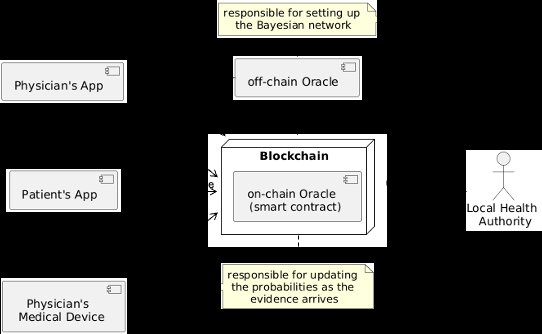
\includegraphics[width=\columnwidth]{Figures/Component_image.pdf}}%
  {\IfFileExists{Figures/Component_image.png}%
    {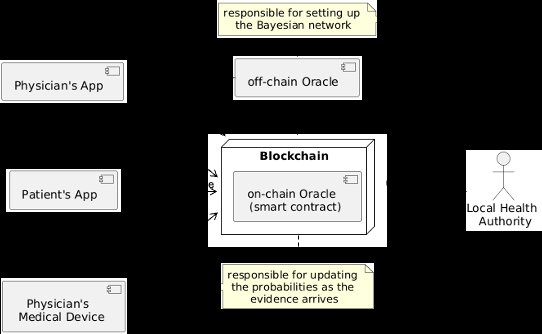
\includegraphics[width=\columnwidth]{Figures/Component_image.png}}%
    {\fbox{\parbox{\columnwidth}{\centering\vspace{1.5cm}
     \texttt{[missing: Figures/Component\_image]}
     \vspace{1.5cm}}}}}
  \caption{SELENE component architecture. The on-chain
  layer hosts four contracts that anchor parameters,
  evidence and posteriors but never execute inference; the
  off-chain oracle operator performs all probabilistic
  computation and commits results through the single
  fixed-width \texttt{OracleController} entry point.}
  \label{fig:component}
\end{figure}

\begin{figure*}[t]
  \centering
  \IfFileExists{Figures/sequence_diagram.pdf}%
  {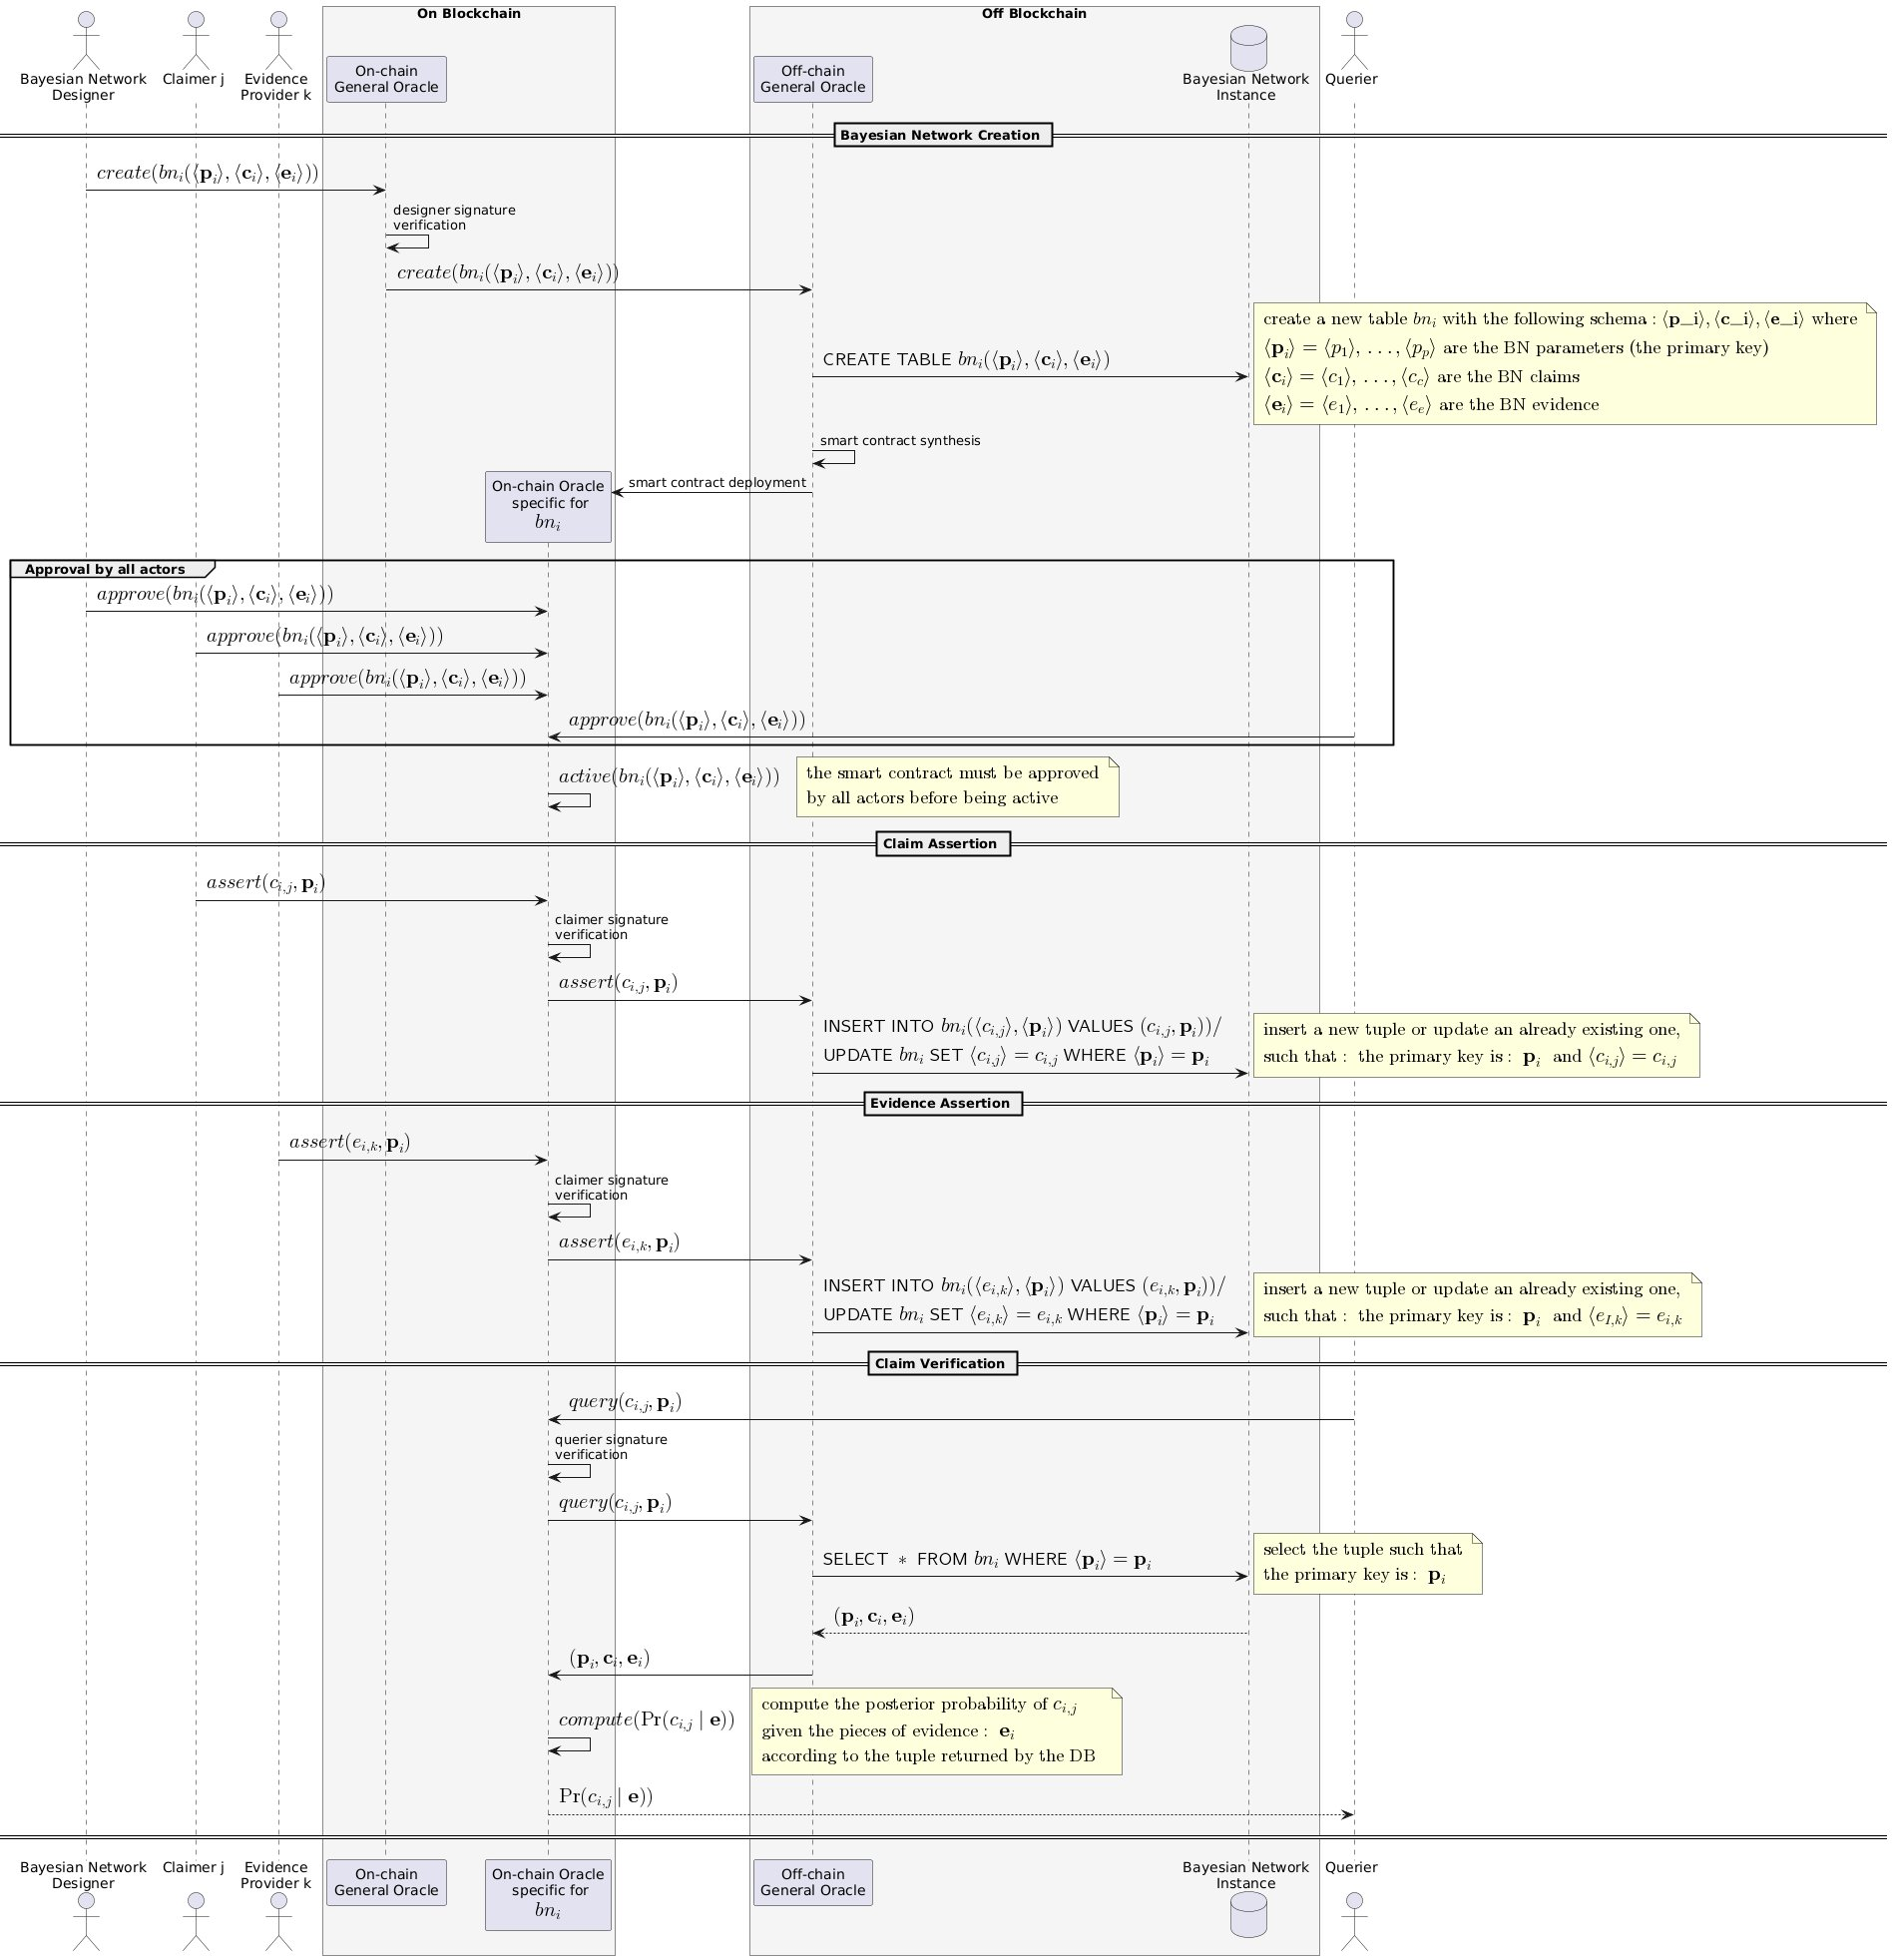
\includegraphics[width=\textwidth,height=0.62\textheight,
     keepaspectratio]{Figures/sequence_diagram.pdf}}%
  {\IfFileExists{Figures/sequence_diagram.png}%
    {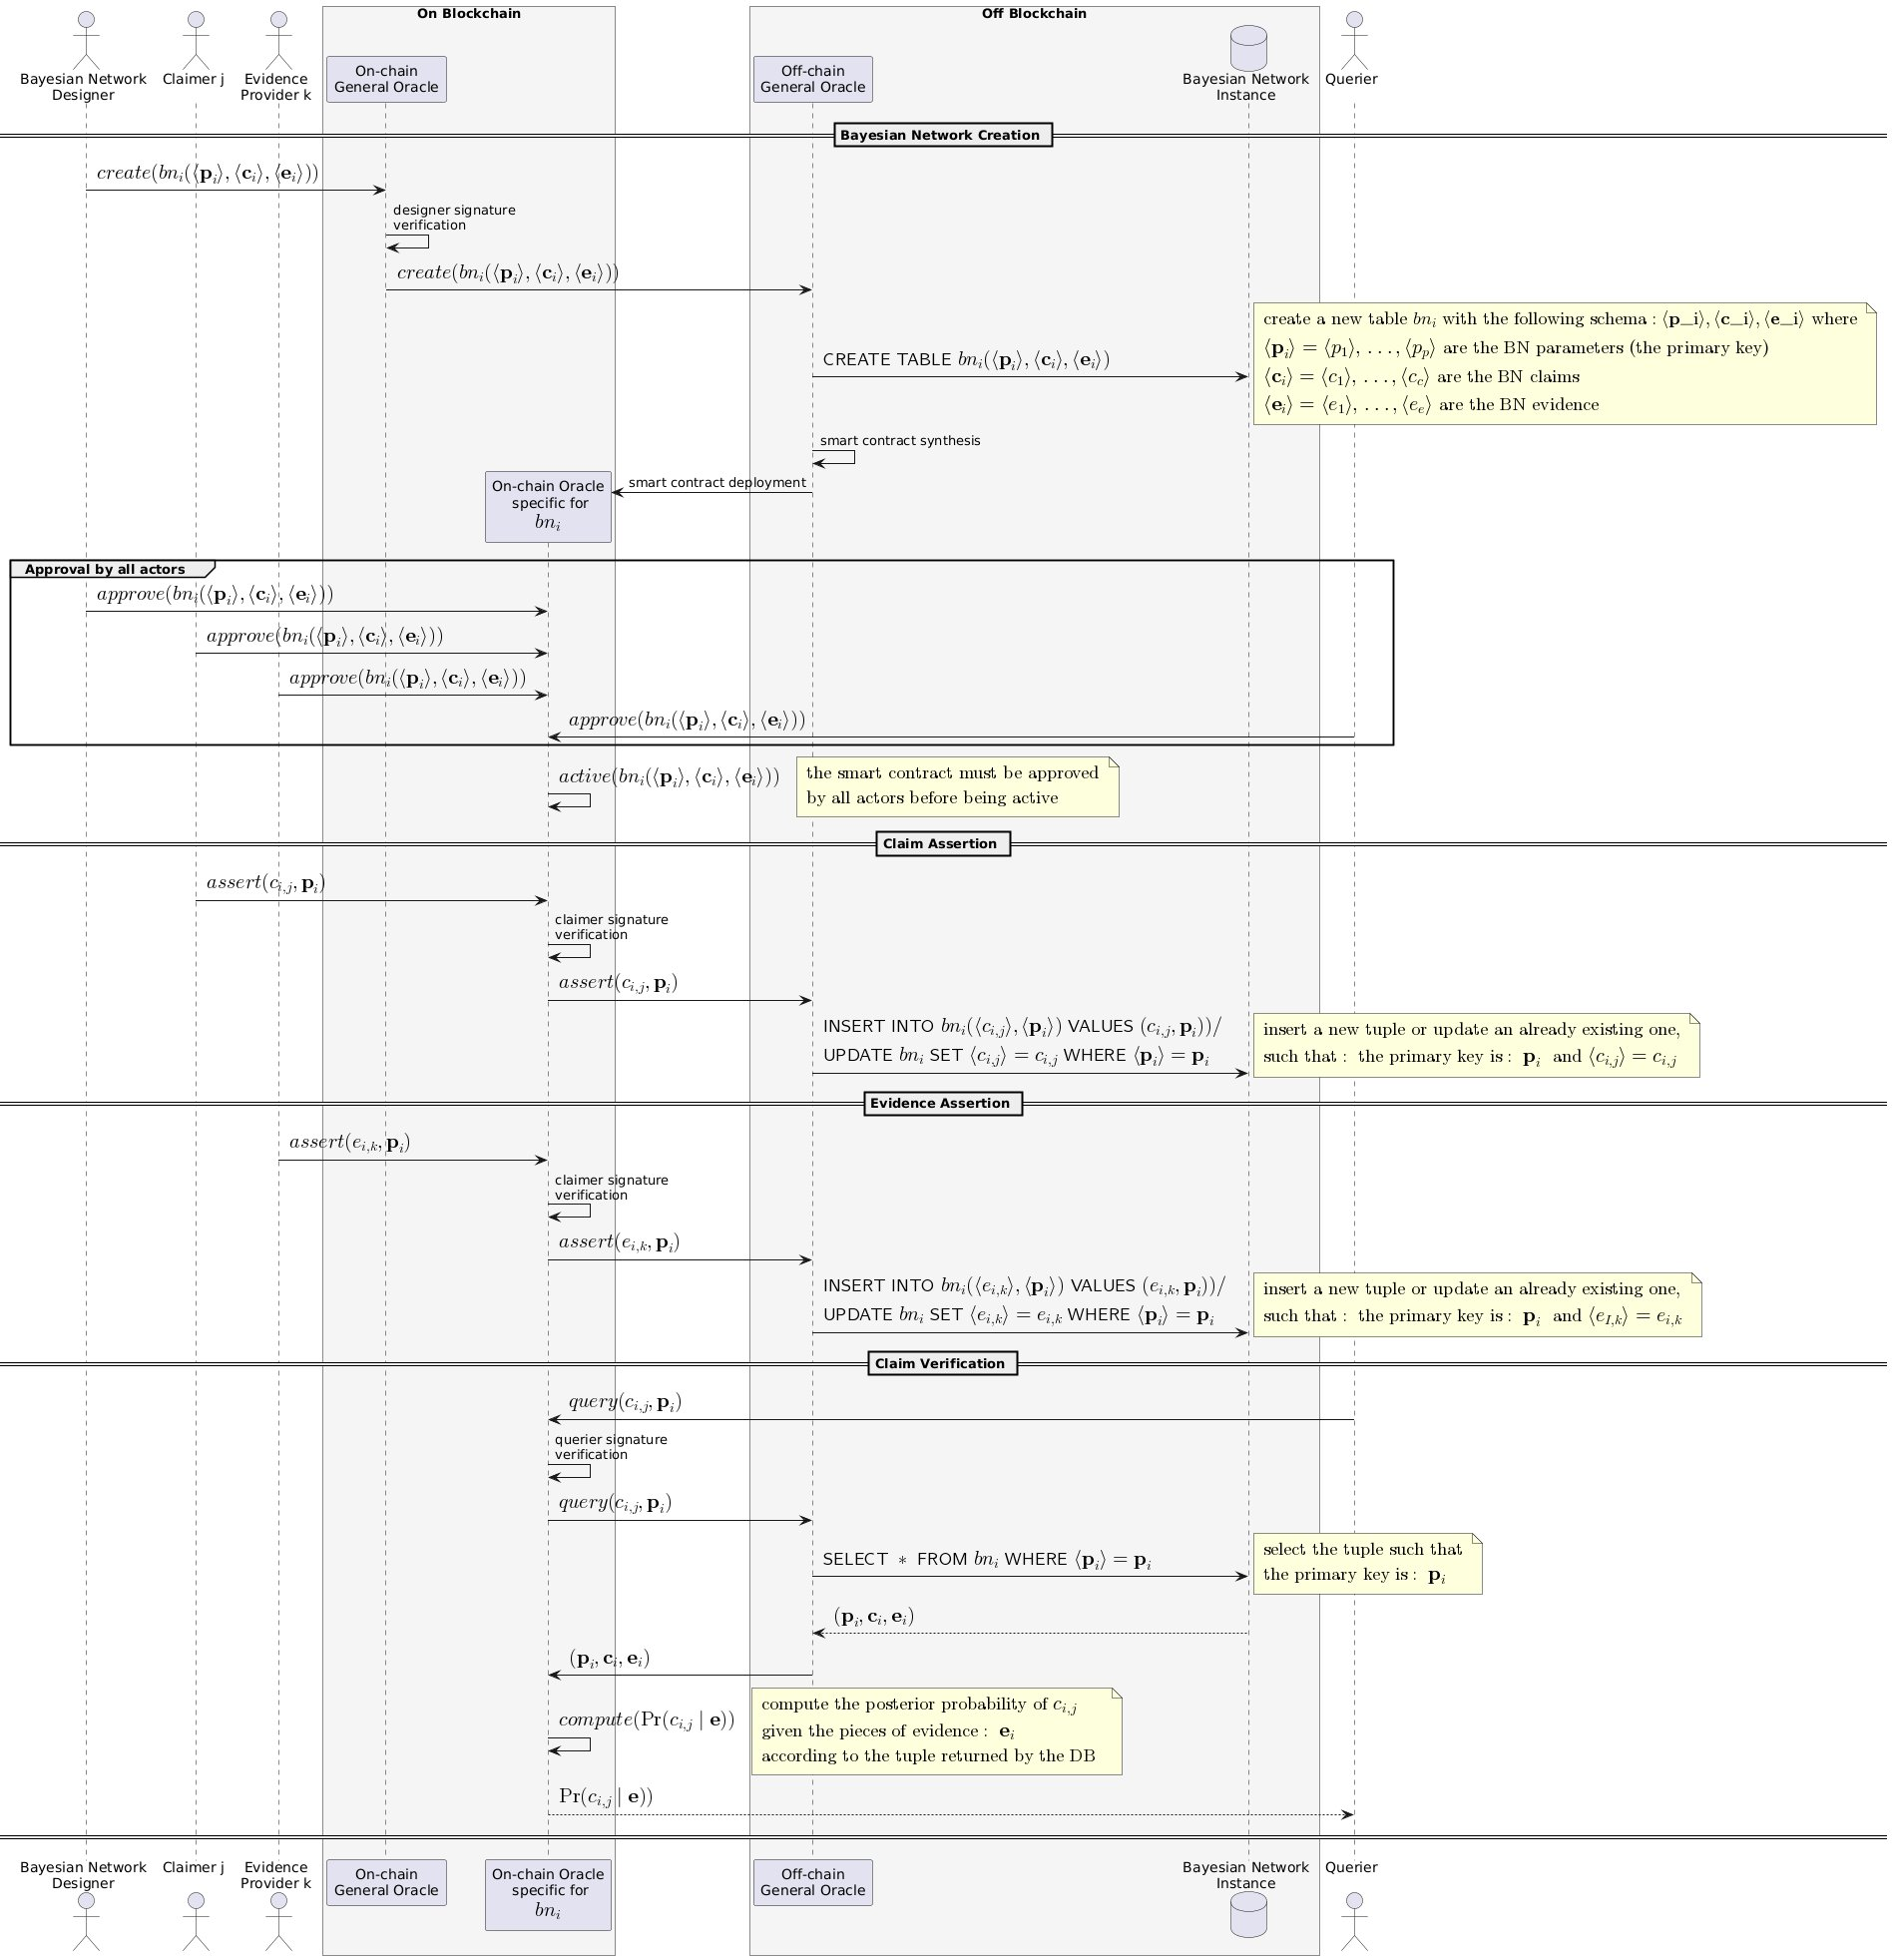
\includegraphics[width=\textwidth,height=0.62\textheight,
       keepaspectratio]{Figures/sequence_diagram.png}}%
    {\fbox{\parbox{\columnwidth}{\centering\vspace{1.5cm}
     \texttt{[missing: Figures/sequence\_diagram]}
     \vspace{1.5cm}}}}}
  \caption{SELENE interaction protocol. Parameter
  anchoring writes the BN to \texttt{CPTStore}; claims are
  opened once and updated as evidence arrives incrementally
  and out of order; the off-chain operator reconstructs the
  BN at block~$b$ and commits posteriors through the
  fixed-width \texttt{submitInference} interface; and any
  party can independently recompute every posterior from
  ledger state alone.}
  \label{fig:sequence}
\end{figure*}


%% ============================================================
\section{Implementation}
\label{sec:implementation}
%% ============================================================

The complete implementation---smart contracts,
off-chain oracle, and experiment scripts---is publicly
available at
\url{https://github.com/S1120957/S_Evidence_BN_Oracle}
(archived release tagged \texttt{v1.0}; a Zenodo DOI
will be minted upon acceptance).

\subsection{On-Chain Contracts}

The on-chain layer is implemented in Solidity~0.8.x
on an Ethereum-compatible EVM, organized into four
contracts with strictly separated responsibilities.
Table~\ref{tab:access-control} summarizes write
permissions.

\textbf{CPTStore} is the sole repository for BN
parameters. It stores prior probabilities
$P(\texttt{PPH}=1)$ and $P(\texttt{PPR}=1)$, and for
each evidence node $E_i\in\mathcal{E}$, the four
conditional entries
$P(E_i=1\mid\texttt{PPH}=i,\texttt{PPR}=j)$,
$i,j\in\{0,1\}$. All values are stored as integers
$\widehat{p}\in\{0,\dots,\texttt{SCALE}\}$ under
$\texttt{SCALE}=10^6$. Every parameter write is
range-checked and emitted as an indexed event,
enabling full reconstruction of the BN parameter
history from the ledger. Write access is restricted
to the deploying account; reads are unrestricted.

\textbf{ClaimRegistry} manages claim state. Each
claim is identified by an internal \texttt{claimId}
and linked to an external key via \texttt{keccak256}.
The registry stores the latest committed posterior
pair and enforces the state machine
$\texttt{None}\to\texttt{Open}\to\texttt{Finalized}$.
The \texttt{Finalized} state is absorbing. Only
\texttt{OracleController} may write to this registry.

\textbf{EvidenceRegistry} maintains an append-only
log of evidence--posterior records. Each entry stores the
\texttt{claimId}, four ternary-coded evidence values in
$\{0,1,2\}$, the two scaled posterior marginals, the
submitting address, and the block number. Code~2 denotes
an unobserved evidence variable. Given this log and the
parameter history in \texttt{CPTStore}, any party can
independently recompute and verify every posterior ever
committed for any claim. Write access is restricted
to \texttt{OracleController}; there is no independent
provider-facing write path in the current prototype.

\textbf{OracleController} is the external entry point for
posterior submission. Its fixed-width
\texttt{submitInference} call accepts
\begin{align*}
(&\texttt{claimId},
 \texttt{gps},\texttt{pc},\texttt{pmd},\texttt{pr},\\
 &\widehat{p}_{\texttt{PPH}},
 \widehat{p}_{\texttt{PPR}},
 \texttt{expectedBnInstanceId}),
\end{align*}
where each evidence value lies in $\{0,1,2\}$.
The controller verifies that the claim is
\texttt{Open}, every evidence value is at most
\texttt{UNOBSERVED}=2, both posterior values lie in
$[0,\texttt{SCALE}]$, the caller is the authorized oracle
operator, and \texttt{expectedBnInstanceId} matches the
current \texttt{CPTStore} parameter fingerprint.
A stale fingerprint therefore causes the transaction to
revert. On success the controller updates
\texttt{ClaimRegistry}, appends the complete
evidence--posterior record to \texttt{EvidenceRegistry},
and emits the corresponding indexed inference event.
No probabilistic inference or CPT traversal occurs
on-chain.

\begin{table}[t]
\centering
\caption{Write permission matrix for SELENE contracts.
Integer overflow is precluded by Solidity~0.8.x
checked arithmetic throughout.}
\label{tab:access-control}
\begin{tabularx}{\columnwidth}{lXl}
\toprule
\textbf{Contract} &
\textbf{Written data} &
\textbf{Caller} \\
\midrule
\texttt{CPTStore}
  & BN priors and CPT entries
  & Deployer \\
\texttt{ClaimRegistry}
  & Claim state and posteriors
  & \texttt{OracleController} \\
\texttt{EvidenceRegistry}
  & Evidence--posterior log
  & \texttt{OracleController} \\
\texttt{OracleController}
  & Inference submissions
  & Authorised oracle \\
\bottomrule
\end{tabularx}
\end{table}

\subsection{Off-Chain Oracle}

The off-chain oracle is implemented in Python~3.x.
Its core component, \texttt{BNOracle}, stores BN
structure and floating-point CPT parameters and
evaluates the posterior pair
$(P(\texttt{PPH}=1\mid e),\,P(\texttt{PPR}=1\mid e))$
via Equation~\eqref{eq:posterior}.

Before each inference run, a synchronisation module
reads all CPT entries from \texttt{CPTStore} via
\texttt{web3.py} and reconstructs the BN from the
current on-chain parameter snapshot at block~$b$.
This ensures submitted posteriors correspond to the
parameter state visible on-chain at reconstruction
time. The block height~$b$ is recorded and included
in the submission event for audit purposes. If
reconstruction fails (RPC timeout or unexpected
contract state), the oracle aborts and logs the
failure without writing to the chain.

The submission pipeline executes five steps:
(i)~reconstruct BN from \texttt{CPTStore} at block~$b$;
(ii)~read current evidence assignment $e^{(t)}$ from
\texttt{EvidenceRegistry};
(iii)~evaluate Equation~\eqref{eq:posterior} over
observed variables, marginalising out $\bot$ entries;
(iv)~encode both marginals as
$\widehat{p}=\texttt{round}(p\cdot\texttt{SCALE})$;
(v)~submit via \texttt{submitInference}, recording
transaction hash and gas used.

Transaction reverts are caught and logged with the
revert reason. The oracle does not retry automatically;
failed submissions require manual inspection. This is
a known limitation of the single-operator design
discussed in Section~\ref{sec:limitations}.

\subsection{Deployment and Experimental Setup}

\textbf{Deployment environment.}
All experiments run on \emph{Sepolia}, the Ethereum
public testnet (EIP-1559 base fees, variable block
packing), providing a realistic public-network validity
check for the gas-predictability claim. All transactions
are publicly verifiable at the addresses in
Table~\ref{tab:contracts}. Reported gas values are
intrinsic execution gas (\texttt{gasUsed}), which is
independent of fluctuating fiat or base-fee pricing.

\begin{table}[t]
\centering
\caption{Definitive Path~A contract deployment on the
Sepolia public testnet. All empirical production-contract
experiments use this single deployment.}
\label{tab:contracts}
\setlength{\tabcolsep}{3pt}
\begin{tabularx}{\columnwidth}{l>{\raggedright\arraybackslash}X}
\toprule
\textbf{Contract} & \textbf{Sepolia address} \\
\midrule
\texttt{CPTStore}
  & {\tiny\texttt{0x6a351aF33059B2a361F44d7E924AEA31BbC8dccc}} \\
\texttt{ClaimRegistry}
  & {\tiny\texttt{0xf16b44768983C68FE418764ec2b740EA7eA14635}} \\
\texttt{EvidenceRegistry}
  & {\tiny\texttt{0xa2e36d0bE698E54cD61d1b0be224fB81ee56d494}} \\
\texttt{OracleController}
  & {\tiny\texttt{0x71668f737d859d977DA13f952f3F0B03DC00ca01}} \\
\bottomrule
\end{tabularx}
\end{table}

\textbf{Toolchain.}
Contracts were compiled and deployed using
Truffle~5.11. Python components interacted with Sepolia
via \texttt{web3.py}~6.x. All dependencies are
version-pinned in \texttt{requirements.txt} and
\texttt{package.json}.

\noindent\textbf{BN parameter configuration.}
All production experiments use the frozen \emph{asymmetric}
configuration of Table~\ref{tab:cpt-values} with priors
$P(\texttt{PPH}{=}1)=0.30$ and $P(\texttt{PPR}{=}1)=0.70$,
chosen to reflect plausible relative signal strengths
rather than elicited clinical estimates; clinical grounding
is future work (Section~\ref{sec:limitations}). The
deployed parameter set was read back from
\texttt{CPTStore} after initialization and is bound to the
fingerprint reported alongside Table~\ref{tab:cpt-values}.

\begin{table}[t]
\centering
\caption{Asymmetric CPT configuration used in non-neutral experiments.
Values are $P(E_i=1\mid\texttt{PPH}=i,\texttt{PPR}=j)$.
Parameters are set to reflect plausible signal strength for each
evidence source in physician-visit verification; clinical validation
against real visit data is identified as future work.}
\label{tab:cpt-values}
\resizebox{\columnwidth}{!}{%
\begin{tabular}{lcccc}
\toprule
& \multicolumn{4}{c}{\textbf{Parent configuration}
  $(\texttt{PPH},\texttt{PPR})$} \\
\cmidrule{2-5}
\textbf{Evidence} &
$(1,0)$ & $(0,1)$ & $(1,1)$ & $(0,0)$ \\
\midrule
\texttt{GPS} &
0.90 & 0.15 & 0.80 & 0.10 \\
\texttt{PC}  &
0.85 & 0.20 & 0.75 & 0.15 \\
\texttt{PMD} &
0.88 & 0.10 & 0.78 & 0.08 \\
\texttt{PR}  &
0.80 & 0.25 & 0.70 & 0.20 \\
\bottomrule
\end{tabular}}
\end{table}

The asymmetric configuration uses
$P(\texttt{PPH}{=}1)=0.30$ and
$P(\texttt{PPR}{=}1)=0.70$.
The final Sepolia deployment was independently read back
after initialization, confirming all 16 CPT entries and
both priors. Its resulting parameter fingerprint is:
\begin{center}
{\tiny\texttt{0x7497ecdac61fd9d1a089b81f068b50d5e136eb9b0d69d320\-c59b15cdb18772e5}}
\end{center}

\noindent\textbf{Experiment profiles.}
Initialization scaling is evaluated for
$N_e\in\{4,8,32\}$ using the parameterized
\texttt{CPTStoreScaling} contract, corresponding to
16, 32, and 128 stored CPT entries. The definitive
production deployment retains four evidence fields.
For the final production gas experiment, 20
\texttt{openClaim} and 20 \texttt{submitInference}
transactions are executed under the asymmetric profile;
the first \texttt{openClaim} measurement is retained in
the raw CSV but excluded from its predefined summary,
yielding $n=19$. Fixed-point fidelity is evaluated under
the frozen asymmetric profile across all $2^4=16$
complete assignments. Lifecycle behaviour is evaluated
using three concurrently open claims and partial ternary
evidence states.


%% ============================================================
\section{Experimental Evaluation}
\label{sec:experimental-analysis}
%% ============================================================

We evaluate SELENE along five dimensions:
(i)~on-chain gas cost as a function of BN size,
contrasted with full on-chain BN inference;
(ii)~fixed-point fidelity and decision consistency;
(iii)~claim lifecycle stability under incremental
out-of-order evidence arrival;
(iv)~the fundamental reliability limits of the evidence
channel and the induced privacy frontier; and
(v)~end-to-end pipeline feasibility on a public
testnet.

\subsection{Gas Scaling with BN Size}
\label{sec:exp-bn-size}

Table~\ref{tab:gas-scaling} reports gas consumption for
three transaction types on Sepolia: per-query operations
(size-invariant) and initialization (scaling with $N_e$).

\begin{table}[t]
\centering
\caption{Measured Sepolia gas consumption.
Per-query measurements use the definitive Path~A production
deployment of Table~\ref{tab:contracts}; values are
mean~$\pm$~population standard deviation.
Twenty measurements were executed for each per-query
operation. Following the predefined measurement protocol,
the first \texttt{openClaim} observation is retained in the
raw log but excluded from its reported summary
($n=19$). Initialization measurements use the auxiliary
parameterized \texttt{CPTStoreScaling} contract.}
\label{tab:gas-scaling}
\begin{tabularx}{\columnwidth}{lXr}
\toprule
\textbf{Operation} &
\textbf{Configuration} &
\textbf{Gas} \\
\midrule
\multicolumn{3}{l}{\emph{Production per-query operations}} \\

\texttt{submitInference}
& fixed-width Path~A interface, $n{=}20$
& $242{,}387.00 \pm 0.00$ \\

\texttt{openClaim}
& fixed-width Path~A interface, $n{=}19$
& $196{,}134.74 \pm 3.68$ \\

\midrule
\multicolumn{3}{l}{\emph{Initialization scaling}} \\

\texttt{CPTStore} init
& $N_e{=}4$ \ (16 entries)
& $895{,}687$ \\

\texttt{CPTStore} init
& $N_e{=}8$ \ (32 entries)
& $1{,}751{,}559$ \\

\texttt{CPTStore} init
& $N_e{=}32$ \ (128 entries)
& $6{,}886{,}791$ \\

\bottomrule
\end{tabularx}
\end{table}

\noindent\textbf{Initialization cost.}
Initialization gas grows linearly with the number of CPT
entries. The parameterized \texttt{CPTStoreScaling}
experiment measured 895{,}687~gas for $N_e=4$
($e=16$ entries), 1{,}751{,}559~gas for $N_e=8$
($e=32$), and 6{,}886{,}791~gas for $N_e=32$
($e=128$). Linear regression gives
\[
  \mathrm{Gas}(e)
  = 39{,}815 + 53{,}492\,e,
\]
with $R^2=1.0000$. Thus, the measured initialization
cost is linear in the number of stored CPT entries over
the tested range.

\noindent\textbf{Per-query cost.}
On the definitive Path~A production deployment,
\texttt{submitInference} consumed exactly
242{,}387~gas in all 20 repetitions
(population standard deviation $0$).
For \texttt{openClaim}, the predefined reporting set
after exclusion of the first measurement contains
$n=19$ observations with
$196{,}134.74 \pm 3.68$~gas
(range 196{,}124--196{,}136).
These measurements characterize the deployed four-evidence
interface. More generally, the contract path is
$O(1)$ with respect to BN inference complexity because
\texttt{OracleController} performs no CPT traversal or
probabilistic inference. The $N_e=4,8,32$ experiment
measures initialization scaling; it should not be
interpreted as three separate per-query measurements.
Figure~\ref{fig:gas-scaling} shows the measured
initialization scaling together with the production
per-query series.

\begin{figure}[t]
  \centering
  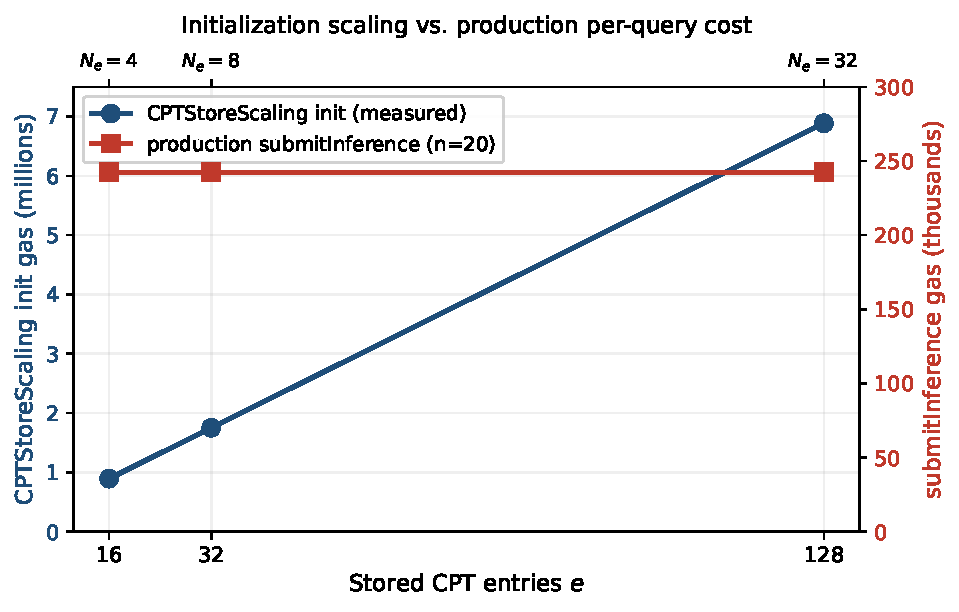
\includegraphics[width=\columnwidth]{Figures/gas_scaling}
  \caption{Measured initialization and per-query gas.
\texttt{CPTStoreScaling} initialization grows linearly
with CPT entries,
$\mathrm{Gas}(e)=39{,}815+53{,}492e$
($R^2=1.0000$), whereas the production
\texttt{submitInference} path consumed exactly
242{,}387~gas in all 20 repetitions. The horizontal
per-query series reflects the fixed-width production
interface; BN-size scaling was measured for initialization.}
  \label{fig:gas-scaling}
\end{figure}

%% Table VI (on-chain BN baseline) cut: no baseline contract was
%% implemented. The comparison is made qualitatively against the
%% size-dependent cost reported by prior on-chain BN work~\cite{naeem2025evidence}.

\subsection{Contrast with On-Chain BN Inference}
\label{sec:exp-comparison}

SELENE's per-query cost is constant in BN size
(Table~\ref{tab:gas-scaling}). This contrasts structurally
with full on-chain BN inference, whose per-query gas grows
with the number of evidence nodes because CPT evaluation and
posterior normalization are executed in the
contract~\cite{naeem2025evidence}. Under SELENE, that size-dependent
arithmetic is moved off-chain and replaced by a fixed-width
posterior commitment; the only BN-size-dependent on-chain
cost is one-time initialization
(Section~\ref{sec:exp-bn-size}). A direct head-to-head gas
comparison against a re-implemented on-chain BN baseline is
left to future work, as it requires a faithful
contemporaneous re-implementation to be meaningful.

\subsection{Fixed-Point Fidelity and Decision Consistency}
\label{sec:exp-fidelity}

We evaluate fixed-point fidelity across all $2^4=16$
complete evidence assignments under the asymmetric CPT
configuration. The resulting 32 posterior marginals span
$[0.002109495,\,0.996448974]$. For each posterior $p$
we compute
$\delta=|p-\widehat{p}/\texttt{SCALE}|$
and evaluate decision consistency at $\tau=0.5$.

\begin{table}[t]
\centering
\caption{Fixed-point encoding fidelity under
$\texttt{SCALE}=10^6$ for all $2^4=16$ complete
evidence assignments (32 posterior marginals).
Near-boundary counts marginals satisfying
$|p-\tau|\leq5{\times}10^{-7}$ at $\tau=0.5$.}
\label{tab:fidelity}
\resizebox{\columnwidth}{!}{%
\begin{tabular}{lrrrr}
\toprule
\textbf{CPT config} &
$\delta_{\max}$ &
$\bar{\delta}$ &
\textbf{Near-bdry} &
\textbf{Inconsist.} \\
\midrule
Asymmetric &
$4.9688{\times}10^{-7}$ &
$2.4394{\times}10^{-7}$ &
0 & 0 \\
\bottomrule
\end{tabular}}
\end{table}

The maximum observed absolute error is
$4.9688\times10^{-7}$, below the theoretical
$5\times10^{-7}$ bound, and the mean absolute error is
$2.4394\times10^{-7}$. None of the 32 marginals falls
within the ambiguity interval around $\tau=0.5$, and all
32 floating-point and fixed-point decisions agree.

To test the decision-consistency criterion directly rather
than relying only on naturally occurring posteriors, we
additionally evaluate 19 synthetic posterior values around
the threshold. All 11 values satisfying
$|p-\tau|>\epsilon$ are decision-consistent, confirming
the soundness direction of
Theorem~\ref{thm:dec-consistency}. Among the eight values
inside or on the boundary
$|p-\tau|\leq\epsilon$, four are inconsistent; all four
occur on the below-threshold side. This empirically
demonstrates that the sufficient margin condition is also
tight, directly answering~RQ3.

\noindent\textbf{Contract boundary checks.}
Nine additional boundary cases verify the Solidity
invariants. Posterior values $0$ and
$\texttt{SCALE}$ are accepted, values above
$\texttt{SCALE}$ revert, evidence code~3 is rejected,
and the designated \texttt{UNOBSERVED} code~2 is
accepted. Submissions to nonexistent or finalized claims,
submissions from unauthorized callers, and submissions
carrying a stale BN fingerprint all revert as expected.
All nine checks pass.

\subsection{Claim Lifecycle Evaluation}
\label{sec:exp-lifecycle}

We evaluate the complete claim lifecycle using three
claims that are opened before any inference submission,
so all three are simultaneously in the \texttt{Open}
state. Evidence is then incorporated incrementally under
three orderings: canonical
$\texttt{GPS}\to\texttt{PC}\to\texttt{PMD}\to\texttt{PR}$,
reverse
$\texttt{PR}\to\texttt{PMD}\to\texttt{PC}\to\texttt{GPS}$,
and a non-canonical gapped ordering
$\texttt{PC}\to\texttt{PR}\to\texttt{GPS}\to\texttt{PMD}$.
Unobserved variables are represented on-chain by
\texttt{UNOBSERVED}=2 and marginalized by the off-chain
inference procedure.

\noindent\textbf{Concurrent lifecycle execution.}
All three claims are verified to be \texttt{Open}
concurrently before the first posterior update.
Across the experiment, 12 staged
\texttt{submitInference} transactions are executed.
Every resulting \texttt{EvidenceRegistry} entry is read
back from chain and independently recomputed; all
12/12 records match, with zero recomputation error for
both posterior marginals.

\noindent\textbf{Gas behaviour.}
Gas depends on storage-update stage rather than evidence
ordering. The first posterior submission for each claim
consumes exactly 242{,}399~gas. Subsequent submissions
consume between 208{,}187 and 208{,}199~gas.
Across all 12 lifecycle submissions the mean is
216{,}743~gas with population standard deviation
14{,}812.50~gas
(range 208{,}187--242{,}399).
At comparable stages the three evidence orderings differ
by at most 12~gas. Thus, the experiment does not support
a single stage-independent update cost; instead, it shows
that evidence ordering has negligible effect once storage
state is controlled.

\noindent\textbf{Posterior convergence.}
Figure~\ref{fig:lifecycle} shows the three trajectories.
The intermediate posterior trajectories differ
substantially with evidence order, as expected for partial
assignments. Once all four evidence variables have been
observed, however, all three claims converge to the same
posterior for the final evidence assignment:
\[
P(\texttt{PPH}{=}1\mid e)=0.8700,
\qquad
P(\texttt{PPR}{=}1\mid e)=0.7596.
\]
This confirms order invariance: the final posterior depends
on the complete evidence assignment rather than its arrival
sequence.

\noindent\textbf{Finalization.}
Each \texttt{finalizeClaim} transaction consumes
42{,}396~gas ($n=3$). All three claims transition to
\texttt{Finalized}, and all three subsequent
\texttt{submitInference} attempts revert with
\texttt{ClaimRegistry: claim not open}. The
\texttt{Finalized} state is therefore empirically
confirmed to be absorbing, completing the answer to~RQ2.

\begin{figure}[t]
  \centering
  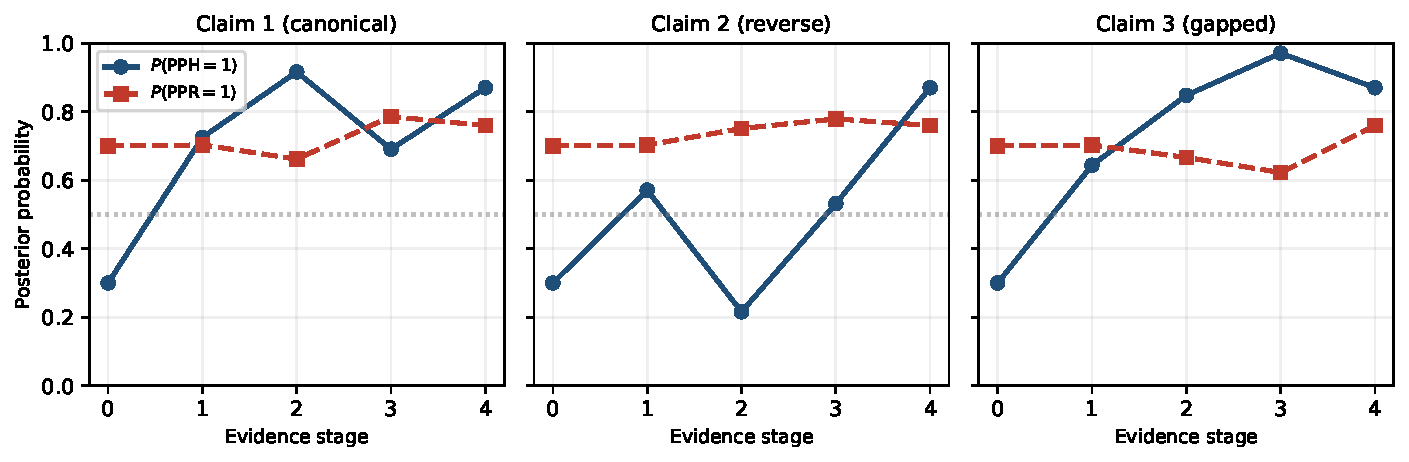
\includegraphics[width=\columnwidth]{Figures/lifecycle_posteriors}
  \caption{Posterior evolution for three concurrently open
claims under canonical, reverse, and gapped evidence
orderings. Unobserved evidence is marginalized at each
stage. Intermediate trajectories differ by arrival order,
but all three converge to
$(P(\texttt{PPH}{=}1),P(\texttt{PPR}{=}1))
=(0.8700,0.7596)$ after the complete evidence assignment
is available.}
  \label{fig:lifecycle}
\end{figure}

\subsection{Parameter Sensitivity}
\label{sec:exp-sensitivity}

Two distinct properties should be separated.
First, the \emph{contract control flow} of
\texttt{openClaim} and \texttt{submitInference} does not
depend on CPT magnitudes: these functions never traverse
or evaluate CPT entries. On the final asymmetric
deployment, \texttt{submitInference} consumed exactly
242{,}387~gas in 20 repeated complete-evidence
submissions, while \texttt{openClaim} consumed
$196{,}134.74\pm3.68$~gas in the predefined
$n=19$ reporting set. BN-size dependence appears instead
in parameter initialization, which scales linearly with
the number of CPT entries.

Second, the \emph{fixed-point error bound} is determined
by $\texttt{SCALE}$. Under
$\texttt{SCALE}=10^6$, the 32 asymmetric-profile
posterior marginals span
$[0.002109495,0.996448974]$ and exhibit a maximum
absolute encoding error of
$4.9688\times10^{-7}$, within the theoretical
$5\times10^{-7}$ bound. Posterior values themselves
remain parameter-dependent; the statement independent
of CPT values concerns the rounding bound, not the
posterior distribution. A full structural
sensitivity study---quantifying how posterior outputs
respond to perturbations of individual CPT entries and to
relaxation of the conditional-independence assumption of
Section~\ref{sec:proposed-methodology}---requires
clinically grounded parameters and is identified as future
work (Section~\ref{sec:limitations}).

\subsection{Fundamental Reliability Limits and the
Privacy Frontier}
\label{sec:exp-risk}

Sections~\ref{sec:exp-bn-size} to~\ref{sec:exp-lifecycle}
characterise what SELENE \emph{does}. This subsection
evaluates what any evidence-based oracle on the same
channel \emph{could} do, by instantiating
Theorems~\ref{thm:risk-ml} and~\ref{thm:risk-chi2} and
Proposition~\ref{prop:privacy} on the asymmetric CPTs of
Table~\ref{tab:cpt-values} with priors
$P(\texttt{PPH}{=}1)=0.3$, $P(\texttt{PPR}{=}1)=0.7$.
These are analytic evaluations of the anchored parameters;
no additional chain interaction is required, and any party
can recompute them from \texttt{CPTStore}.

For this configuration $p_{\max}=0.49$, attained at
$(\texttt{PPH},\texttt{PPR})=(0,1)$.

\textbf{Evidence sufficiency.}
Table~\ref{tab:risk-bounds} reports both bounds as
evidence accumulates.
With no evidence the $\chi^2$ bound reduces to
$1-\sqrt{p_{\max}}=0.300$, exactly the risk of guessing
from the prior. Each additional observation lowers the
attainable risk floor, reaching $0.055$ on the full
evidence set: even a perfect oracle consuming all four
signals misclassifies at least $5.5\%$ of claims under
these CPTs. This is a statement about evidence quality,
not about SELENE.

The two measures behave differently, as
Section~\ref{sec:theory-limits} anticipated. The
maximal-leakage bound is tighter for $|S|\le2$ but
collapses to the vacuous value $0$ at $|S|\ge3$, whereas
the $\chi^2$ bound remains informative throughout. Neither
dominates, consistent with the general observation
in~\cite{esposito2024lower}.

\begin{table}[t]
\centering
\caption{Fundamental lower bounds on oracle Bayesian risk
as a function of the observed evidence set, computed from
the anchored CPTs of Table~\ref{tab:cpt-values}
($p_{\max}=0.49$, $0$--$1$ loss). Values are for the most
informative subset of each size; ``---'' marks a bound that
has degenerated to the trivial value $0$. Minimum
admissible evidence counts follow from
Corollary~\ref{cor:gating}.}
\label{tab:risk-bounds}
\begin{tabularx}{\columnwidth}{cXrrr}
\toprule
$|S|$ &
\textbf{Most informative subset} &
$\mathcal{L}(W{\to}X_S)$ &
\textbf{ML bd.} &
$\chi^2$ \textbf{bd.} \\
\midrule
0 & $\emptyset$              & 0.000 & 0.510 & 0.300 \\
1 & \texttt{PMD}             & 0.588 & 0.118 & 0.141 \\
2 & \texttt{GPS,PMD}         & 0.669 & 0.044 & 0.095 \\
3 & \texttt{GPS,PC,PMD}      & 0.747 & ---   & 0.068 \\
4 & all four                 & 0.762 & ---   & 0.055 \\
\bottomrule
\end{tabularx}
\end{table}

\textbf{Proposed risk-gated execution.}
Applying Corollary~\ref{cor:gating} to the $\chi^2$
column yields a candidate admission rule for a future
deployment. A tolerance
of $\tau_{\mathrm{risk}}=0.15$ is met by a single
well-chosen observation; $\tau_{\mathrm{risk}}=0.10$
requires at least two; $0.075$ requires three; and
$0.06$ requires all four. A tolerance below $0.055$ is
\emph{unattainable} with this evidence set at any cost,
which is actionable design information: it says the CPTs,
not the contract, are the binding constraint. Because $\mathcal{S}^{\star}$ is a fixed predicate over
the observed-evidence pattern, it could be enforced with
constant-size contract logic. The present Path~A
prototype does not implement this gate; the analysis here
evaluates the rule offline from the anchored CPTs.

\textbf{Privacy frontier.}
Proposition~\ref{prop:privacy} quantifies the cost of
perturbing evidence before publication. With
$\chi^2(W,X)=0.822$ on the full evidence set, a
privatisation level $\lambda=0.25$---corresponding to an
$(\varepsilon,0)$-LDP budget of
$\varepsilon=\log 3\approx1.10$---raises the risk floor
from $0.055$ to $0.232$, i.e.\ it caps achievable accuracy
at $76.9\%$ rather than $94.5\%$. At $\lambda=0.5$ the
bound reaches $1-\sqrt{p_{\max}}=0.300$: the evidence
carries no information and the oracle can do no better
than the prior. Figure~\ref{fig:risk-bounds} plots both
relationships.

\begin{figure}[t]
  \centering
  \includegraphics[width=\columnwidth]{Figures/risk_bounds}
  \caption{Fundamental limits on oracle reliability for the
  SELENE evidence channel. (a)~Lower bound on Bayesian
  risk as evidence accumulates; the shaded band spans
  subsets of equal size and the dotted line marks an
  example tolerance $\tau_{\mathrm{risk}}=0.10$.
  (b)~Privacy--reliability frontier under
  $\mathrm{BSC}(\lambda)$ privatisation; the shaded region
  is unachievable by any oracle.}
  \label{fig:risk-bounds}
\end{figure}

This frontier is what
Section~\ref{sec:limitations} previously described only
qualitatively: it converts ``committing evidence to a
public ledger is a privacy risk'' into a quantitative
statement about how much reliability a given privacy
budget costs, and it does so without reference to any
particular inference implementation, answering~RQ4.

\subsection{End-to-End Feasibility on a Public Testnet}
\label{sec:exp-e2e}

All results above were obtained by executing the complete
pipeline---contract deployment, CPT initialization, claim
opening, off-chain BN reconstruction from
\texttt{CPTStore}, posterior submission, and read-back
verification---against the Sepolia public testnet under
live EIP-1559 base-fee conditions, rather than a local
emulator. Across the full experiment suite (parameter
initialization, 20 \texttt{openClaim} and 20
\texttt{submitInference} per-query measurements, 16
fixed-point fidelity assignments, the nine contract
boundary checks, and the three-claim partial-evidence
lifecycle), every transaction confirmed and every
committed posterior matched its off-chain counterpart on
read-back, confirming
that the architecture is deployable on production-grade
public infrastructure. The contract addresses in
Table~\ref{tab:contracts} allow independent verification
of all reported transactions via a public block explorer.


%% ============================================================
\section{Discussion}
\label{sec:results-discussion}
%% ============================================================

\subsection{Answering the Research Questions}

\textbf{RQ1 --- Gas-predictable per-query cost.}
On the definitive production deployment,
\texttt{submitInference} consumed exactly
242{,}387~gas in all 20 repetitions (population standard
deviation $0$), and \texttt{openClaim}
$196{,}134.74\pm3.68$~gas ($n=19$). The contract path is
$O(1)$ with respect to BN inference complexity because it
performs no CPT traversal or probabilistic arithmetic; the
only BN-size-dependent cost is one-time initialization,
which scales linearly at 53{,}492~gas per CPT entry
($R^2=1.0000$) in the parameterized scaling experiment.

\textbf{RQ2 --- Lifecycle support without
redeployment.}
Three concurrently open claims complete the full
lifecycle without redeployment under three evidence
orderings and partial ternary evidence. All 12 on-chain
evidence records are independently reconstructed with
zero recomputation error, all three orderings converge to
the same complete-evidence posterior
$(0.8700, 0.7596)$, and all three post-finalization
submissions revert. Update gas is stage-dependent
(first write 242{,}399~gas; subsequent overwrites
208{,}187--208{,}199~gas) but effectively invariant to
evidence ordering at comparable stages.

\textbf{RQ3 --- Fixed-point decision consistency.}
For $\texttt{SCALE}=10^6$, no decision inconsistencies
are observed across the 32 posterior marginals, with
maximum encoding error $4.9688\times10^{-7}$ against the
theoretical bound of $5\times10^{-7}$. The dedicated
boundary sweep confirms both directions of
Theorem~\ref{thm:dec-consistency}: all 11 synthetic
posteriors with $|p-\tau|>\epsilon$ are consistent, and
four of the eight inside or on the boundary are not, all
on the below-threshold side. The encoding-error bound
depends only on $\texttt{SCALE}$, not on CPT values.

\textbf{RQ4 --- Fundamental reliability limits.}
Independently of implementation, the evidence channel
anchored in \texttt{CPTStore} imposes a risk floor of
$0.055$ under the studied CPTs: no oracle consuming these
four signals can classify claims more accurately than
$94.5\%$. The floor is monotone in the observed evidence
set, which yields a proposed admission rule
(Corollary~\ref{cor:gating}) evaluated offline in this
work, and it degrades in a
closed-form way under privatisation, rising to $0.232$ at
an $\varepsilon{\approx}1.10$ local differential-privacy
budget. This reframes CPT elicitation as the binding
constraint on oracle quality: contract-level engineering
cannot recover reliability that the evidence channel does
not contain.

\subsection{Design Trade-offs}

The core design choice---off-chain inference with
on-chain parameter anchoring---introduces a clear
trade-off between gas efficiency and runtime
correctness enforcement.

\textbf{Auditability vs.\ real-time enforcement.}
SELENE provides post-hoc auditability: any party can
reconstruct and verify any posterior from on-chain
state. However, a malicious oracle operator can
submit an incorrect posterior detectable only after
the fact. In healthcare settings where decisions are
acted upon immediately, post-hoc detection may be
insufficient. This is the most consequential
limitation of the current design.

\textbf{Structural fixity vs.\ adaptability.}
BN structure is fixed at deployment. Adding a new
evidence source requires redeployment and resets all
claim history. In a live healthcare setting where
evidence types evolve, this rigidity is a practical
barrier.

\textbf{Single claim variable encoding.}
The current design uses two independent root nodes
(\texttt{PPH} and \texttt{PPR}). A cleaner
alternative is a single binary root variable
$C\in\{0,1\}$, which would halve the number of root
configurations, reduce CPT size by half, and
eliminate the marginal independence assumption between
claim variables. We retain the two-root design for
compatibility with~\cite{naeem2025evidence} but recommend the
single-variable encoding for future deployments.

\subsection{Limitations}
\label{sec:limitations}

\textbf{Synthetic CPT parameters.}
All experiments use either neutral or heuristically
specified CPT values. Gas and fidelity results are
independent of CPT values by construction, but
posterior quality depends critically on parameter
correctness. Clinically grounded CPT elicitation from
real physician-visit data is necessary before any
clinical deployment.

\textbf{Limited BN size range.}
BN sizes beyond 32~evidence nodes are not tested. The
$O(N_e)$ initialization bound is consistent with
measurements at 4, 8, and 32~nodes but is not
validated beyond this range.

\textbf{Single oracle operator.}
The current prototype uses a single trusted oracle
operator. Contention, failure, and adversarial
behaviour of the oracle are not evaluated. Gas and
latency overhead of a multi-operator committee design
remain unmeasured.

\textbf{Privacy exposure.}
Committing binary evidence assignments to a public ledger
may expose patient-linked information. Under GDPR and
HIPAA, this requires either a permissioned deployment,
evidence commitment via cryptographic commitment schemes,
or local perturbation of evidence before submission.
Proposition~\ref{prop:privacy} quantifies the cost of the
third option, but the analysis assumes an idealised binary
symmetric perturbation applied independently per evidence
bit; correlated leakage across claims for the same patient,
and the composition of privacy budgets over repeated
submissions, are not modelled here.


%% ============================================================
\section{Conclusion}
\label{sec:conclusion}
%% ============================================================

This paper addresses a fundamental tension in
BN-based oracle design: on-chain inference preserves
verifiability but does not scale; off-chain inference
scales but severs the verifiability link.
SELENE resolves this by treating the blockchain as an
authenticated parameter and audit plane rather than
an inference engine. BN structure and CPTs are
anchored on-chain; inference executes off-chain; and
every evidence assignment, posterior output, and state
transition is committed as an immutable,
reconstructible transcript. Correctness is auditable
post-hoc from ledger state alone.

Five concrete results are established. First, the
fixed-width production inference path is $O(1)$ with
respect to BN inference complexity and consumed exactly
242{,}387~gas across 20 repeated
\texttt{submitInference} transactions on Sepolia;
initialization scales linearly at 53{,}492~gas per CPT
entry ($R^2=1.0000$) over 4, 8, and 32 evidence nodes.
Second, fixed-point encoding under
$\texttt{SCALE}=10^6$ has a maximum observed absolute
error of $4.9688\times10^{-7}$ across 32 posterior
marginals, below the theoretical
$5\times10^{-7}$ bound, with no decision
inconsistencies; a dedicated boundary sweep additionally
confirms the soundness and tightness of the decision-margin
criterion. Third, three concurrently open claims support
incremental, out-of-order partial evidence and converge to
the same final posterior
$(0.8700,0.7596)$ once the complete evidence assignment is
available; all 12 evidence records are independently
reconstructed exactly, and all three post-finalization
updates revert. Fourth, the inference transcript is
reconstructible from the anchored parameter state,
evidence--posterior records, and indexed events. Fifth,
casting oracle operation as Bayesian estimation yields an
implementation-independent risk floor of $0.055$ for the
studied evidence channel and a closed-form
privacy--reliability frontier. The associated risk-gating
predicate is proposed and analytically evaluated but is
not implemented in the current contracts.

These results hold under explicit scope conditions:
BN structure is fixed at deployment, evidence
variables are binary, CPT parameters are synthetic
in this evaluation, and the oracle operator is a
single trusted party. These conditions define the
boundary of this contribution and the frontier for
future work.

Three directions are prioritised. The most
consequential is oracle centralization: a single
operator can submit incorrect posteriors detectable
only post-hoc. The immediate next step is a
multi-operator committee design with on-chain
detection of divergent submissions. The second
direction is clinical CPT validation: evaluating SELENE
with CPTs elicited from real physician-visit data is
necessary before any clinical deployment. The third
direction is privacy-preserving inference: integrating
zero-knowledge proofs for posterior verification without
evidence disclosure would simultaneously address the
privacy constraint and the runtime correctness gap, and
would move the deployment off the
privacy--reliability frontier of
Proposition~\ref{prop:privacy} rather than merely along
it. A fourth direction follows from
Section~\ref{sec:theory-limits}: the risk bounds
currently gate execution using a fixed evidence-set
predicate, but the same divergences support
\emph{adaptive} evidence acquisition, in which an IoT node
selects the next most informative sensor and halts as soon
as the certified risk crosses the tolerance.

SELENE demonstrates that interpretable, auditable
BN-based oracle decisions are practically deployable
without gas costs that scale with model complexity.
The architecture is explicit about what it does not
yet provide---runtime correctness enforcement,
clinical parameter validation, and privacy
preservation---and these define the starting point
for the next stage of this work.



%% ============================================================
\appendices
\section{Proofs}
\label{app:proofs}
%% ============================================================

Throughout, $\epsilon=1/(2\cdot\texttt{SCALE})$,
$\widehat{p}=\texttt{round}(p\cdot\texttt{SCALE})$, and
$\mathcal{W}=\{0,1\}^2$ is the space of claim
configurations. We write $P_{X_S\mid W}$ for the evidence
channel of Definition~\ref{def:evidence-channel} and
$p_{\max}=\max_{w}P_W(w)$.

\subsection{Proof of Theorem~\ref{thm:rounding}}
\label{app:proof-rounding}

\begin{proof}
Write $t=p\cdot\texttt{SCALE}\in[0,\texttt{SCALE}]$. By
definition of round-half-to-even (or any rounding rule to
the nearest integer), $\widehat{p}$ is an integer
minimising $|t-\widehat{p}|$, hence
$|t-\widehat{p}|\le\tfrac12$. Dividing by
$\texttt{SCALE}>0$,
\[
  \left|p-\frac{\widehat{p}}{\texttt{SCALE}}\right|
  = \frac{|t-\widehat{p}|}{\texttt{SCALE}}
  \le \frac{1}{2\cdot\texttt{SCALE}} = \epsilon .
\]
Attainment: take $p=(2k+1)/(2\cdot\texttt{SCALE})$ for any
integer $0\le k<\texttt{SCALE}$; then
$t=k+\tfrac12$ and $|t-\widehat p|=\tfrac12$ exactly, so
the bound is met with equality. Finally
$\widehat{p}\in\{0,\dots,\texttt{SCALE}\}$ because
$t\in[0,\texttt{SCALE}]$ and rounding is monotone.
\end{proof}

\subsection{Proof of Theorem~\ref{thm:dec-consistency}}
\label{app:proof-consistency}

\begin{proof}
\emph{(i) Soundness.} Let
$\tilde{p}=\widehat{p}/\texttt{SCALE}$ and suppose
$|p-\tau|>\epsilon$. By Theorem~\ref{thm:rounding},
$|p-\tilde{p}|\le\epsilon$. If $p>\tau+\epsilon$ then
$\tilde{p}\ge p-\epsilon>\tau$, so both indicators in
Definition~\ref{def:dec-consistency} equal $1$. If
$p<\tau-\epsilon$ then $\tilde{p}\le p+\epsilon<\tau$, so
both indicators equal $0$. In either case $p$ is
decision-consistent.

\emph{(ii) Tightness.} Fix $\texttt{SCALE}$ and
$\tau\in(0,1)$, and choose the integer
$k=\lceil \tau\cdot\texttt{SCALE}\rceil$ so that
$k/\texttt{SCALE}\ge\tau$. Consider
$p=\tau-\delta$ for $\delta>0$ arbitrarily small with
$p\cdot\texttt{SCALE}\ge k-\tfrac12$. Then
$\widehat{p}=k$ and
$\tilde{p}=k/\texttt{SCALE}\ge\tau$, whence
$\mathbb{1}[\tilde{p}\ge\tau]=1$ while
$\mathbb{1}[p\ge\tau]=0$: the encoded and floating-point
decisions differ. Such $p$ satisfies
$|p-\tau|=\delta\le\epsilon$ by construction, so
inconsistency does occur inside the interval and the
criterion in~(i) cannot be widened.

\emph{Minimum scale.} If a deployment guarantees margin
$|p-\tau|\ge m$, then by~(i) consistency holds whenever
$m>\epsilon=1/(2\cdot\texttt{SCALE})$, i.e.\ whenever
$\texttt{SCALE}>1/(2m)$.

\emph{(Asymmetry.)} The construction in~(ii) produces a
failure only from below, because
Definition~\ref{def:dec-consistency} uses the closed
condition $\ge\tau$: rounding can promote a value just
below $\tau$ to exactly $\tau$, but cannot demote a value
that already satisfies $p\ge\tau$ past the threshold
without violating Theorem~\ref{thm:rounding}. This
one-sidedness is confirmed empirically in
Section~\ref{sec:exp-fidelity}.
\end{proof}

\subsection{Proof of Lemmas~\ref{lem:smallball}
and~\ref{lem:markov}}
\label{app:proof-lemmas}

\begin{proof}[Proof of Lemma~\ref{lem:smallball}]
Under the $0$--$1$ loss, $\ell(W,\hat{w})\in\{0,1\}$, so
for $\rho\in(0,1]$ the event $\{\ell(W,\hat w)<\rho\}$
coincides with $\{\ell(W,\hat w)=0\}=\{W=\hat w\}$.
Therefore
\[
  L_W(\rho)
  =\sup_{\hat w\in\mathcal{W}} P_W(W=\hat w)
  =\max_{w\in\mathcal{W}} P_W(w)
  =p_{\max},
\]
which does not depend on $\rho$ in $(0,1]$.
\end{proof}

\begin{proof}[Proof of Lemma~\ref{lem:markov}]
Since $\ell\ge0$, Markov's inequality gives, for every
$\rho>0$,
\begin{align*}
  \mathbb{E}\bigl[\ell(W,\widehat W)\bigr]
  &\;\ge\; \rho\,
     P_{W\widehat W}\bigl(\ell(W,\widehat W)\ge\rho\bigr)\\
  &= \rho\Bigl(1-P_{W\widehat W}
     \bigl(\ell(W,\widehat W)<\rho\bigr)\Bigr),
\end{align*}
using $P(\ell\ge\rho)=1-P(\ell<\rho)$.
\end{proof}

\subsection{Proof of Theorems~\ref{thm:risk-ml}
and~\ref{thm:risk-chi2}}
\label{app:proof-risk-bounds}

Both proofs instantiate the general framework
of~\cite{esposito2024lower} at $\rho=1$, which is the
largest admissible value under the $0$--$1$ loss and hence
yields the tightest bound obtainable from
Lemma~\ref{lem:markov}.

\begin{proof}[Proof of Theorem~\ref{thm:risk-ml}]
Let $\varphi$ be any estimator, so that
$W-X_S-\widehat W$ is a Markov chain. Applying the
maximal-leakage probability bound
of~\cite{esposito2024lower} to the event
$E=\{\ell(W,\widehat W)<\rho\}$,
\[
  P_{W\widehat W}(E)
  \;\le\; e^{\mathcal{L}(W\to\widehat W)}\,L_W(\rho)
  \;\le\; e^{\mathcal{L}(W\to X_S)}\,L_W(\rho),
\]
where the second inequality is the data-processing
inequality for maximal leakage along
$W-X_S-\widehat W$. Substituting into
Lemma~\ref{lem:markov} and using
Lemma~\ref{lem:smallball},
\[
  \mathbb{E}\bigl[\ell(W,\widehat W)\bigr]
  \;\ge\;
  \rho\Bigl(1-p_{\max}e^{\mathcal{L}(W\to X_S)}\Bigr).
\]
The right-hand side is independent of $\varphi$, so it
lower bounds the infimum $R_B$. Setting $\rho=1$ gives the
claim. The closed form of $\mathcal{L}$ for discrete
alphabets is
$\mathcal{L}(W\to X_S)=\log\sum_x\max_w
P_{X_S\mid W=w}(x)$~\cite{esposito2024lower}.

Finally, the bound involves $P_W$ only through
$p_{\max}$: $\mathcal{L}$ depends on $P_W$ solely through
its support, so any two priors sharing a support and a
maximum probability give the identical bound.
\end{proof}

\begin{proof}[Proof of Theorem~\ref{thm:risk-chi2}]
Take the Hellinger divergence $\mathcal{H}_p$ generated by
$\phi_p(x)=(x^p-1)/(p-1)$ and specialise the
$\phi$-divergence risk bound of~\cite{esposito2024lower}
to $p=2$, for which $\mathcal{H}_2=\chi^2$. That bound
states
\[
  R_B \;\ge\;
  \rho\Bigl(
    1-L_W(\rho)^{\frac{p-1}{p}}
     \bigl((p-1)\mathcal{H}_p(W,X_S)+1\bigr)^{\frac1p}
  \Bigr).
\]
The two data-processing steps required to remove the
dependence on $\varphi$---namely
$\mathcal{H}_p(W,\widehat W)\le\mathcal{H}_p(W,X_S)$ and
$L_W(\widehat W,\rho)\le L_W(\rho)$---are admissible
because the governing functional is non-decreasing in each
argument. With $p=2$, Lemma~\ref{lem:smallball} and
$\rho=1$,
\[
  R_B \;\ge\;
  1-\sqrt{p_{\max}\bigl(\chi^2(W,X_S)+1\bigr)} .
\qedhere
\]
\end{proof}

\subsection{Proof of Proposition~\ref{prop:privacy}}
\label{app:proof-privacy}

\begin{proof}
Let $Z_S$ be obtained from $X_S$ by passing each bit
independently through $K=\mathrm{BSC}(\lambda)$, so that
$W-X_S-Z_S-\widehat W$ is a Markov chain and
$Z_S$ is generated by the tensor product $K^{\otimes|S|}$.
For $1\le p\le 2$ the SDPI coefficient of a binary
symmetric channel is
$\eta_p(K)=(1-2\lambda)^2$, and $\eta_p$ tensorises,
$\eta_p(P_{X_S},K^{\otimes|S|})=\eta_p(P_{X_1},K)
\le(1-2\lambda)^2$~\cite{esposito2024lower}. Hence the
strong data-processing inequality gives
\[
  \mathcal{H}_2(W,Z_S)
  \;\le\; (1-2\lambda)^2\,\mathcal{H}_2(W,X_S)
  \;=\; (1-2\lambda)^2\,\chi^2(W,X_S).
\]
Substituting this contracted quantity for
$\chi^2(W,X_S)$ in the proof of
Theorem~\ref{thm:risk-chi2} yields
\[
  R_B^{\mathrm{priv}}
  \;\ge\;
  1-\sqrt{p_{\max}\bigl((1-2\lambda)^2\chi^2(W,X_S)+1
  \bigr)} .
\]
For the privacy statement, $\mathrm{BSC}(\lambda)$ with
$\lambda=1/(1+e^{\varepsilon})$ is
$(\varepsilon,0)$-locally differentially
private~\cite{esposito2024lower}; inverting,
$\varepsilon=\log((1-\lambda)/\lambda)$. Substituting this
into the display gives the trade-off curve as an explicit
function of the privacy budget.

Two sanity checks: at $\lambda=0$ ($\varepsilon\to\infty$,
no privatisation) the bound reduces to
Theorem~\ref{thm:risk-chi2}; at $\lambda=\tfrac12$
($\varepsilon=0$, complete privatisation) it reduces to
$1-\sqrt{p_{\max}}$, the risk of estimating $W$ from the
prior alone.
\end{proof}


%% ============================================================
%% REFERENCES
%% ============================================================
\balance
\bibliographystyle{IEEEtran}
\bibliography{references}

\end{document}
